\documentclass[11pt]{article}

\usepackage{fontspec}
\usepackage{graphicx}
\usepackage{amsmath}
\usepackage{amssymb}
\usepackage{eso-pic}
\usepackage{hyperref}
\usepackage{listings}
\usepackage{enumerate}
\usepackage{setspace}
\usepackage[parfill]{parskip}
\usepackage{fancyhdr}
\usepackage[a4paper, left=2cm, right=2cm, top=2cm, bottom=2.5cm]{geometry}
\usepackage[useregional]{datetime2}
\usepackage{xcolor}
\usepackage{booktabs}
\usepackage{float}
\usepackage{array}

\lstset{
    basicstyle=\ttfamily\small,
    breaklines=true,
    breakatwhitespace=true,
    commentstyle=\color{gray}\itshape,
    showstringspaces=false,
    columns=flexible,
    keepspaces=true,
    frame=single,
    framesep=4pt,
    rulecolor=\color{gray!40},
    backgroundcolor=\color{gray!10},
    xleftmargin=0pt,
}

\definecolor{myrulecolor}{RGB}{0,0,97}

\IfFontExistsTF{TeX Gyre Termes}{\setmainfont{TeX Gyre Termes}}{}

\makeatletter
\def\@maketitle{%
  \newpage
  \null
  \vspace*{-3em}
  \begin{center}
    {\LARGE\bf\scshape \@title \par}
    \vskip 1.5em
    Group: 26 \\
    Team Member: Jiachen Shi, Pengyu Wang, Minyi Zhu
  \end{center}
  \par
  \vskip 1.5em}
\makeatother

\fancypagestyle{myfancy}{%
    \fancyhf{}
    \fancyhead{}
    \fancyfoot[R]{\thepage}
}

\fancypagestyle{plain}{%
    \fancyhf{}
    \renewcommand{\headrulewidth}{0pt}
    \fancyfoot[R]{\selectfont\thepage}
}

\title{DD2356 VT26\\
Project Report: \\Graph analytics: PageRank learning implementation}

\setcounter{page}{1}
\begin{document}
\pagestyle{myfancy}
\maketitle
\vspace*{-13em}
\IfFileExists{KTH_logo_bla.eps}{%
  \hspace*{-3em}\includegraphics[width=0.1\paperwidth]{KTH_logo_bla.eps}%
}{}
\vspace*{3.5em}

\begin{center}
    \textcolor{myrulecolor}{\rule{\textwidth}{1.5pt}}
\end{center}
\setstretch{1.15}

\begin{abstract}
\noindent
We implement and evaluate parallel PageRank on three CPU platforms (Colab,
KTH JupyterHub, and Dardel), covering OpenMP, MPI, hybrid MPI+OpenMP,
profiling-driven optimizations, and an OpenMP target-offload implementation
evaluated on an NVIDIA H100 MIG device. Profiling places the iterative kernel
at $0.10$ FLOP/Byte, deep in the memory-bound region. OpenMP reaches
$4.32\times$ peak speedup at $T{=}16$ on Dardel. In the formal two-node
Dardel MPI run, the balanced synthetic graph scales to $2.98\times$ at
$P{=}8$ before full-vector \texttt{MPI\_Allgatherv} traffic limits
efficiency, while the much smaller \texttt{polblogs} graph is
communication-bound from $P{=}2$. Persistent GPU data mapping improves the
naive target implementation by $1.7762\times$, although a same-server hybrid
CPU run remains $3.2500\times$ faster at the tested graph size. All formal
parallel-result variants verify against the serial reference within $10^{-6}$.
\end{abstract}

\section{Introduction}
\label{sec:intro}

PageRank~\cite{pagerank} is the canonical sparse-matrix graph-analytics
kernel: each power-iteration step multiplies a dense rank vector by a sparse
transition matrix, exposing irregular memory access and global reductions. We
parallelise the kernel with OpenMP, MPI, and hybrid MPI+OpenMP, add an OpenMP
target-offload implementation, and evaluate the CPU paths on three
heterogeneous platforms (Colab, KTH JupyterHub, and Dardel). GPU offloading
is evaluated separately on a confirmed NVIDIA H100 MIG target allocation.
Together these measurements quantify how memory bandwidth, MPI collective
latency, graph topology, and accelerator data mapping determine the best
configuration. The contributions of this report are:

\begin{itemize}\itemsep0pt
    \item A verified serial C/C++ baseline used as correctness and performance reference.
    \item OpenMP, MPI, and hybrid MPI+OpenMP implementations evaluated on the target CPU systems.
    \item Two profiling-driven optimizations and a confirmed-device OpenMP GPU-offloading path.
    \item Strong and weak scaling studies, plus correctness validation against the serial reference.
\end{itemize}

\section{Background and Problem Description}
\label{sec:background}

PageRank assigns a stationary score $r\in\mathbb{R}^{N}$ to every vertex of a
directed graph via the power iteration
\begin{equation}
\label{eq:pagerank}
r^{(k+1)}_{v}\;=\;\underbrace{\tfrac{1-d}{N}}_{\texttt{base}}
\;+\;\underbrace{\tfrac{d}{N}\!\!\sum_{u:\,d_{\mathrm{out}}(u)=0}\!\!r^{(k)}_{u}}_{\texttt{dang}}
\;+\;d\!\sum_{u\to v}\!\frac{r^{(k)}_{u}}{d_{\mathrm{out}}(u)},
\end{equation}
with $d=0.85$ (damping), $r^{(0)}_{v}=1/N$, and the convergence test
$\lVert r^{(k+1)}-r^{(k)}\rVert_{1}<\varepsilon$, $\varepsilon=10^{-10}$,
capped at $1000$ iterations. The three terms correspond directly to the
\texttt{base}, \texttt{dang}, and inner-sum variables in the serial kernel:
\texttt{base} is loop-invariant, \texttt{dang} is one global reduction over
$r^{(k)}$ per iteration, and the third term is the only per-edge work.

The graph is stored in CSR keyed by \emph{incoming} edges:
\texttt{row\_ptr[v]\,..\,row\_ptr[v+1]-1} lists the sources $u$ that
contribute to $v$, and \texttt{inv\_out\_degree[u]} is precomputed once so
the inner loop multiplies instead of divides. This layout gives the
destination loop no write-write contention, so OpenMP and the MPI
destination-block decomposition both parallelise it directly, and reduces
dangling handling to a single \texttt{MPI\_Allreduce} per iteration. The
access pattern is streaming over \texttt{col\_idx} but a random read into
$r^{(k)}$ and \texttt{inv\_out\_degree}, which, combined with the low
arithmetic intensity of Eq.~\ref{eq:pagerank}, places the kernel deep in the
memory-bound region of the roofline (Sec.~\ref{sec:profiling}).

\section{Design and Implementation}
\label{sec:design}

\subsection{Serial Baseline}
\label{subsec:serial}

The serial implementation (\texttt{serial/pagerank\_serial.c}, $\sim 380$
lines, \texttt{gcc -O2 -lm}) realises Eq.~\ref{eq:pagerank} directly:
CSV rows are parsed once, vertex names are hashed to dense ids
$0\ldots N{-}1$ via a chained hash table, the incoming-edge CSR is built
in two passes, and \texttt{inv\_out\_degree[u]} is precomputed so the
inner update is a multiply rather than a division. The same binary on
the same input is deterministic, so cross-platform PR-time differences
in Table~\ref{tab:serial-baseline} isolate microarchitecture effects.
A \texttt{PR\_REPEAT} environment variable repeats the kernel in-process
to amplify gprof/perf sampling; the per-run timing always divides by the
repeat count.

\begin{table}[H]
\centering
\caption{Serial PageRank baseline: PR-kernel time (seconds) on
representative datasets. Iterations are deterministic across platforms.}
\label{tab:serial-baseline}
\small
\begin{tabular}{lrrrrr}
\toprule
Dataset & $N$ & $M$ & Colab & KTH & Dardel \\
\midrule
polblogs (directed)              & 1\,224   & 19\,090     & 0.01740 & 0.00240 & 0.00345 \\
NCAA\_football (directed)        & 570      & 1\,537      & 0.00018 & 0.00006 & 0.00009 \\
lesmis (undirected)              & 77       & 1\,016      & 0.00017 & 0.00011 & 0.00012 \\
dolphins (undirected)            & 62       & 636         & 0.00015 & 0.00006 & 0.00009 \\
synthetic\_large (directed)      & 100\,000 & 2\,000\,000 & 0.15645 & 0.04014 & 0.08934 \\
\bottomrule
\end{tabular}
\end{table}

\subsection{OpenMP Parallelization}
\label{subsec:openmp}

The three per-iteration passes from Sec.~\ref{subsec:serial} are
parallelised with \texttt{\#pragma omp parallel for}~\cite{openmp}: the
dangling-mass scan and the $L_1$ convergence test use
\texttt{reduction(+:...)} with \texttt{schedule(static)} (constant work
per index), while the sparse incoming-edge update uses
\texttt{schedule(dynamic, 256)} because the in-degree varies widely
across destination vertices in real graphs. All threads share the
immutable CSR (\texttt{row\_ptr}, \texttt{col\_idx},
\texttt{inv\_out\_degree}) and read-only $r^{(k)}$; per-iteration
writes target disjoint \texttt{pr\_new[v]} entries and require no
atomics. A compile switch \texttt{-DPR\_UPDATE\_SCHEDULE\_STATIC}
replaces the dynamic schedule with a static one, enabling the schedule
ablation in Sec.~\ref{sec:wang-optimization}. Thread placement uses
\texttt{OMP\_PLACES=cores OMP\_PROC\_BIND=close} for one thread per
physical core and first-touch NUMA locality. The node-name hash table was
generalised from a fixed $10^{5}$-entry static pool to heap allocation so
the same binary handles the $2{\times}10^{5}$-vertex weak-scaling input.

\subsection{MPI Decomposition and Communication}
\label{subsec:wang-mpi}

The MPI~\cite{mpi} implementation uses a destination-node block
decomposition. For a graph with $N$ vertices and $P$ MPI ranks, rank $r$
owns a contiguous vertex interval $[start_r,end_r)$ and computes only
the corresponding entries of the next PageRank vector. The graph uses
the same incoming-edge CSR layout as the serial baseline. To keep the
first distributed-memory version simple and readily verifiable, every
rank stores the full CSR graph and current PageRank vector, while only
the newly computed block \texttt{pr\_new[start:end]} is rank-local.

The graph is loaded on rank 0 and distributed with \texttt{MPI\_Bcast}.
Each PageRank iteration performs one scalar \texttt{MPI\_Allreduce} for
global dangling-node mass, one scalar \texttt{MPI\_Allreduce} for the
global $L_1$ convergence difference, and one \texttt{MPI\_Allgatherv}
to assemble the full next PageRank vector on every rank. Its cost is
therefore modelled as
\[
T_{\mathrm{iter}}(P) \approx T_{\mathrm{comp}}\left(\frac{M}{P}\right)
    + 2T_{\mathrm{allreduce}}(P)
    + T_{\mathrm{allgatherv}}(N,P).
\]
This model predicts communication-bound behaviour for small graphs, or
at sufficiently many ranks when full-vector gathering dominates the
reduced local sparse update.

\subsection{Hybrid MPI+OpenMP}
\label{subsec:wang-hybrid}

The hybrid implementation reuses the MPI destination-block decomposition
and adds OpenMP parallelism inside each rank. Each rank owns a contiguous
vertex interval and parallelises its dangling-node mass, sparse update,
and convergence passes with OpenMP reductions where appropriate. The
sparse loop uses \texttt{schedule(dynamic, 256)} to distribute irregular
incoming-edge work. The communication contract remains two scalar
\texttt{MPI\_Allreduce}s and one full-vector \texttt{MPI\_Allgatherv} per
iteration, allowing the same binary to evaluate different $(P,N)$ rank
and thread splits at a fixed total CPU-worker budget.

\subsection{OpenMP GPU Offloading}
\label{subsec:wang-gpu}

The accelerator path uses OpenMP target offloading and provides two
variants. The \texttt{naive} baseline maps graph and PageRank data for
target kernels, whereas the \texttt{persistent} variant establishes an
outer target-data region and retains the CSR arrays and ping-pong
PageRank buffers on device across all iterations. Dangling-mass and
convergence reductions are also executed on the target. Formal GPU runs
set \texttt{PR\_REQUIRE\_DEVICE=1}; a host fallback is therefore a
failed measurement rather than an accepted offload result. Since the
Dardel CPU allocation did not provide an accelerator job, formal device
measurements used the DD2356 Small GPU server with an NVIDIA H100
\texttt{MIG 1g.10gb} allocation, alongside a same-server hybrid
\texttt{4x2} CPU control.

\section{Experimental Methodology}
\label{sec:methodology}

Table~\ref{tab:systems} lists the three CPU target systems, spanning a
single-core commodity node (Colab), an interactive multi-socket host
(KTH JupyterHub), and scheduled Dardel compute nodes~\cite{dardel}.
Serial and hotspot/perf measurements use \texttt{gcc -O2 -lm}.

\begin{table}[H]
\centering
\caption{CPU target systems.}
\label{tab:systems}
\small
\begin{tabular}{@{}p{0.12\textwidth}p{0.26\textwidth}p{0.26\textwidth}p{0.26\textwidth}@{}}
\toprule
 & Colab & KTH JupyterHub & Dardel \\
\midrule
OS                & Ubuntu 22.04 & Ubuntu 22.04 & SUSE Linux \\
CPU               & Intel Xeon @ 2.20\,GHz & Intel Xeon Platinum 8480C & AMD EPYC 7742 \\
Max clock         & 2.20\,GHz & 3.80\,GHz & 2.25\,GHz \\
Cores             & 1 phys / 1 log & 112 phys / 224 log (2$\times$56) & 128 phys / 256 log (2$\times$64) \\
Memory            & 12\,GB & 2.0\,TB & 250\,GB \\
Serial compiler   & gcc 11.4.0 & gcc 12.3.0 & gcc 7.5.0 \\
\bottomrule
\end{tabular}
\end{table}

We use two dataset suites. The \emph{correctness suite} is the nine
course-provided graphs (for example, polblogs, dolphins, and lesmis, in
the style of the SNAP collection~\cite{snap}; $34$--$1224$ vertices),
used for serial and parallel verification. The \emph{performance suite}
adds deterministic generated inputs: \path{synthetic_large_directed.csv}
($N=10^{5}$, $M=2{\times}10^{6}$, $10.68$\,MiB working set) drives
serial profiling, and \path{synthetic_100k_1m.csv}
($N=10^{5}$, $M=10^{6}$) drives MPI, hybrid, optimization, and GPU
experiments. Weak scaling uses generated graphs with $12\,500$ vertices
and $125\,000$ edges per rank, reaching $200\,000$ vertices and
$2\,000\,000$ edges at 16 ranks. The skewed optimization input directs
$80\%$ of non-cycle edges to a contiguous hot destination region to
expose thread-level load imbalance.

Each PR-kernel timing is the iteration loop body between two
\texttt{clock\_gettime(CLOCK\_MONOTONIC)} calls. General scaling cells
use five back-to-back repetitions. The formal optimization ablation uses
one warmup followed by ten verified repetitions per variant and layout.
The formal Dardel MPI experiment is Slurm job \texttt{20957663} on the
\texttt{main} partition: multi-rank cells run across two compute nodes
(\texttt{nid001120} and \texttt{nid001121}), with placement captured
outside timed intervals. Earlier single-node Dardel MPI measurements are
retained only as diagnostic records and are not used in the final tables.
The GPU measurements require confirmed target execution on the H100 MIG
device; their hybrid comparison is performed on the same server.

Hotspot profiling rebuilds with \texttt{-O2 -pg} and sets
\texttt{PR\_REPEAT=20} for gprof/perf sampling; per-run kernel time
always divides total time by \texttt{PR\_REPEAT}. The \texttt{perf stat}
event set (\path{cycles,instructions,cache-references,cache-misses,}
\path{L1-dcache-load-misses,LLC-load-misses}) is sampled in
\texttt{all} scope on KTH and user-only
(\texttt{:u}) on Dardel; these scopes are kept separate in analysis.
Correctness uses \texttt{verify/verify\_correctness.c} (per-node maximum
absolute/relative difference plus Top-$K$ rank consistency), with a
verifier tolerance of $10^{-6}$.

\section{Performance Profiling and Analysis}
\label{sec:profiling}

The serial baseline is profiled with \texttt{gprof}~\cite{gprof} and
\texttt{perf stat}~\cite{perf} on both a representative course graph
(\texttt{polblogs.csv}) and the performance-suite large graph. These
measurements establish the memory-bound behaviour against which the
parallel implementations are evaluated.

\paragraph{Hotspot localisation.}
Table~\ref{tab:gprof-large} summarises the gprof flat profile on the
large graph. The \texttt{pagerank} kernel accounts for
$87.5\%$--$92.3\%$ of total time on all three platforms; CSV parsing
and node-name hashing are measurable one-time setup costs, so the
optimization budget belongs to the iterative kernel.

\begin{table}[H]
\centering
\caption{gprof flat profile on \texttt{synthetic\_large\_directed.csv},
$PR\_REPEAT=20$. Columns are percentages of total runtime.}
\label{tab:gprof-large}
\small
\begin{tabular}{lrrrr}
\toprule
Platform & \texttt{pagerank} & \texttt{load\_csv} & \texttt{sht\_get\_or\_insert} & \texttt{iv\_push} \\
\midrule
Colab  & 92.27 & 4.00 & 3.47 & 0.27 \\
KTH    & 87.50 & 4.55 & 6.82 & 1.14 \\
Dardel & 90.87 & 2.17 & 5.22 & 0.87 \\
\bottomrule
\end{tabular}
\end{table}

\paragraph{Memory-bound diagnosis.}
The inner loop \texttt{s += pr[u] * inv\_out\_degree[u]} performs $2$
FLOPs per edge while moving $20$ bytes ($4$\,B \texttt{col\_idx}
streamed plus $8$\,B \texttt{pr[u]} and $8$\,B
\texttt{inv\_out\_degree[u]} fetched at random positions), giving an
arithmetic intensity of $0.10$ FLOP/Byte. With modern CPU ridge points
in the $5$--$10$ FLOP/Byte range, the kernel is deep in the
memory-bound roofline region. \texttt{perf stat} corroborates this:
IPC drops from $3.31/2.67$ on cache-resident \texttt{polblogs.csv}
(KTH/Dardel) to $1.67$ on the large graph for both platforms; L1-miss
rate per $10^{3}$ instructions rises from $2.1/12.4$ to
$168.5/185.1$. Effective bandwidth on KTH is $18.07$\,GB/s versus a
DDR5 peak near $300$\,GB/s per socket, consistent with random-access
rather than streaming behaviour. Speedups must therefore come primarily
from reduced memory traffic, improved reuse, or amortised overhead.

\paragraph{Amdahl ceiling and kernel-time regime.}
Wall-clock time decomposes as $T_{\mathrm{load}} + T_{\mathrm{PR}} +
T_{\mathrm{save}}$, but only $T_{\mathrm{PR}}$ is parallelised. The PR
fraction on \texttt{polblogs.csv} is $45.2\%$ on Colab, $60.0\%$ on
KTH, and $24.2\%$ on Dardel, capping end-to-end speedup at
$1.82\times$, $2.50\times$, and $1.32\times$ respectively. The
performance results therefore report PR-kernel time as their meaningful
parallel metric. For \texttt{polblogs}, even that kernel is already
millisecond-scale, so the formal MPI runs become communication-dominated
before adding ranks can produce useful kernel-time speedup.

\section{Correctness Evaluation}
\label{sec:correctness}

All parallel outputs were validated against the serial PageRank reference
using \path{verify/verify_correctness.c} at tolerance $10^{-6}$.
The verifier keys vectors by node name and checks numerical difference and
Top-$K$ rank consistency, allowing implementations to use different
internal vertex ordering. Table~\ref{tab:correctness-summary} summarises
the validated coverage. The GPU entries are formal target executions:
\path{omp_is_initial_device()} recorded execution on the NVIDIA H100
MIG device rather than host fallback.

\begin{table}[H]
\centering
\caption{Correctness coverage for the reported parallel implementations.}
\label{tab:correctness-summary}
\scriptsize
\begin{tabular}{@{}p{0.18\textwidth}p{0.22\textwidth}p{0.42\textwidth}p{0.10\textwidth}@{}}
\toprule
Implementation & Dataset scope & Configuration & Result \\
\midrule
OpenMP & 9 course datasets & CPU thread-parallel implementation & PASS \\
MPI & 9 course datasets & Dardel reference/correctness runs & PASS \\
MPI & Strong/weak scaling inputs & Formal two-node Dardel, $P=1,2,4,8,16$ & PASS \\
MPI & Strong/weak scaling inputs & School cluster, $P=1,2,4,8,16$ & PASS \\
Hybrid MPI+OpenMP & 2 cluster datasets & Fixed 16 workers, \texttt{1x16} through \texttt{16x1} & PASS \\
Optimization variants & Regular and skewed synthetic graphs & Four variants, nine layouts, ten repetitions & PASS \\
OpenMP target GPU & 9 course datasets and timed synthetic graph & H100 MIG, device execution required & PASS \\
\bottomrule
\end{tabular}
\end{table}

Observed differences are at machine-precision scale; for example, timed
GPU measurements on the synthetic comparison graph have maximum error
$1.02\times10^{-20}$. The formal MPI scaling data and every reported
optimization cell also pass the $10^{-6}$ tolerance.

\section{Scaling Evaluation}
\label{sec:wang-scaling}

\subsection{MPI Strong Scaling on Formal Dardel Two-Node Run}
\label{subsec:mpi-dardel-strong}

The formal Dardel MPI scaling run was submitted as Slurm job
\texttt{20957663} on the \texttt{main} partition. For every multi-rank
row, ranks were explicitly balanced across compute nodes
\texttt{nid001120} and \texttt{nid001121}. Table~\ref{tab:mpi-dardel-polblogs}
shows that the small \texttt{polblogs.csv} input is dominated by
collective synchronization once more than one rank is used.

\begin{table}[H]
\centering
\caption{Formal two-node Dardel MPI strong scaling on
\texttt{polblogs.csv} (directed), five repetitions per row.}
\label{tab:mpi-dardel-polblogs}
\small
\begin{tabular}{rrrrrr}
\toprule
Ranks & PR (s) & Comm frac. & Speedup & Efficiency & Imbalance \\
\midrule
1  & 0.002364 & 0.0463 & 1.000000 & 1.000000 & 1.000 \\
2  & 0.003274 & 0.9144 & 0.722008 & 0.361004 & 1.887 \\
4  & 0.003406 & 0.9637 & 0.694110 & 0.173528 & 3.129 \\
8  & 0.003346 & 0.9805 & 0.706557 & 0.088320 & 4.412 \\
16 & 0.003732 & 0.9896 & 0.633474 & 0.039592 & 4.536 \\
\bottomrule
\end{tabular}
\end{table}

The larger balanced synthetic input performs enough local sparse work to
benefit from distribution through eight ranks. As
Table~\ref{tab:mpi-dardel-synth} shows, it reaches $2.976714\times$
speedup at $P=8$, after which collective traffic raises communication
fraction to $0.7600$ and reduces speedup at $P=16$.

\begin{table}[H]
\centering
\caption{Formal two-node Dardel MPI strong scaling on
\texttt{synthetic\_100k\_1m.csv} (directed), five repetitions per row.}
\label{tab:mpi-dardel-synth}
\small
\begin{tabular}{rrrrrr}
\toprule
Ranks & PR (s) & Comm frac. & Speedup & Efficiency & Imbalance \\
\midrule
1  & 0.036330 & 0.0395 & 1.000000 & 1.000000 & 1.000 \\
2  & 0.020386 & 0.1462 & 1.782080 & 0.891040 & 1.035 \\
4  & 0.012707 & 0.3017 & 2.859025 & 0.714756 & 1.044 \\
8  & 0.012205 & 0.5257 & 2.976714 & 0.372089 & 1.047 \\
16 & 0.014107 & 0.7600 & 2.575258 & 0.160954 & 1.051 \\
\bottomrule
\end{tabular}
\end{table}

Since synthetic in-edge imbalance stays at most $1.051$, the high-rank
decline is driven primarily by collectives rather than poor local work
partitioning.

\begin{figure}[H]
\centering
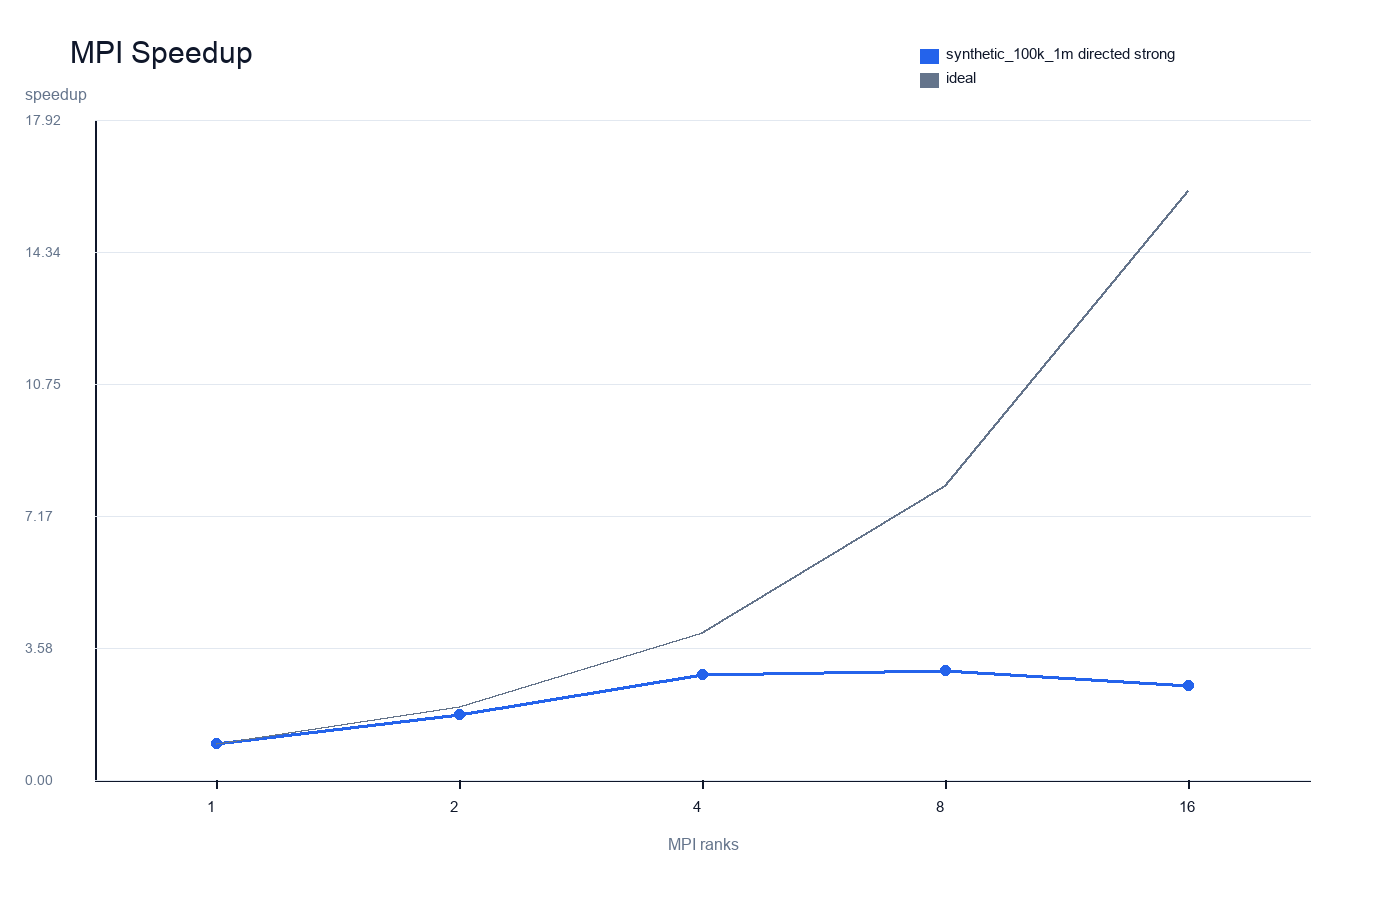
\includegraphics[width=0.48\textwidth]{results/figures/dardel_multinode_strong/mpi_speedup.png}
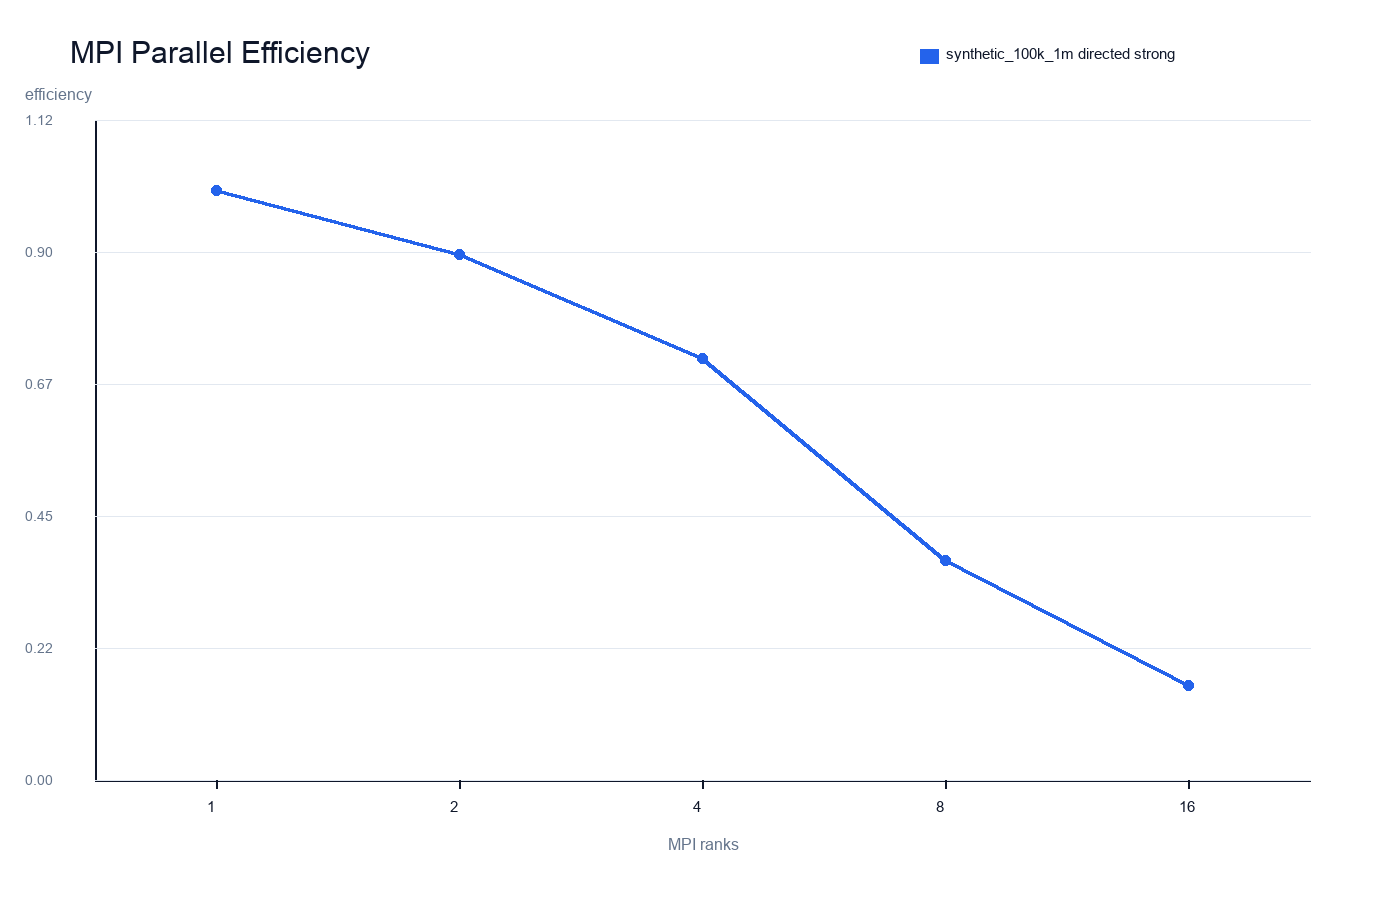
\includegraphics[width=0.48\textwidth]{results/figures/dardel_multinode_strong/mpi_efficiency.png}
\caption{Formal Dardel two-node MPI speedup and efficiency on
\texttt{synthetic\_100k\_1m.csv}.}
\label{fig:dardel-mpi-speedup}
\end{figure}

\begin{figure}[H]
\centering
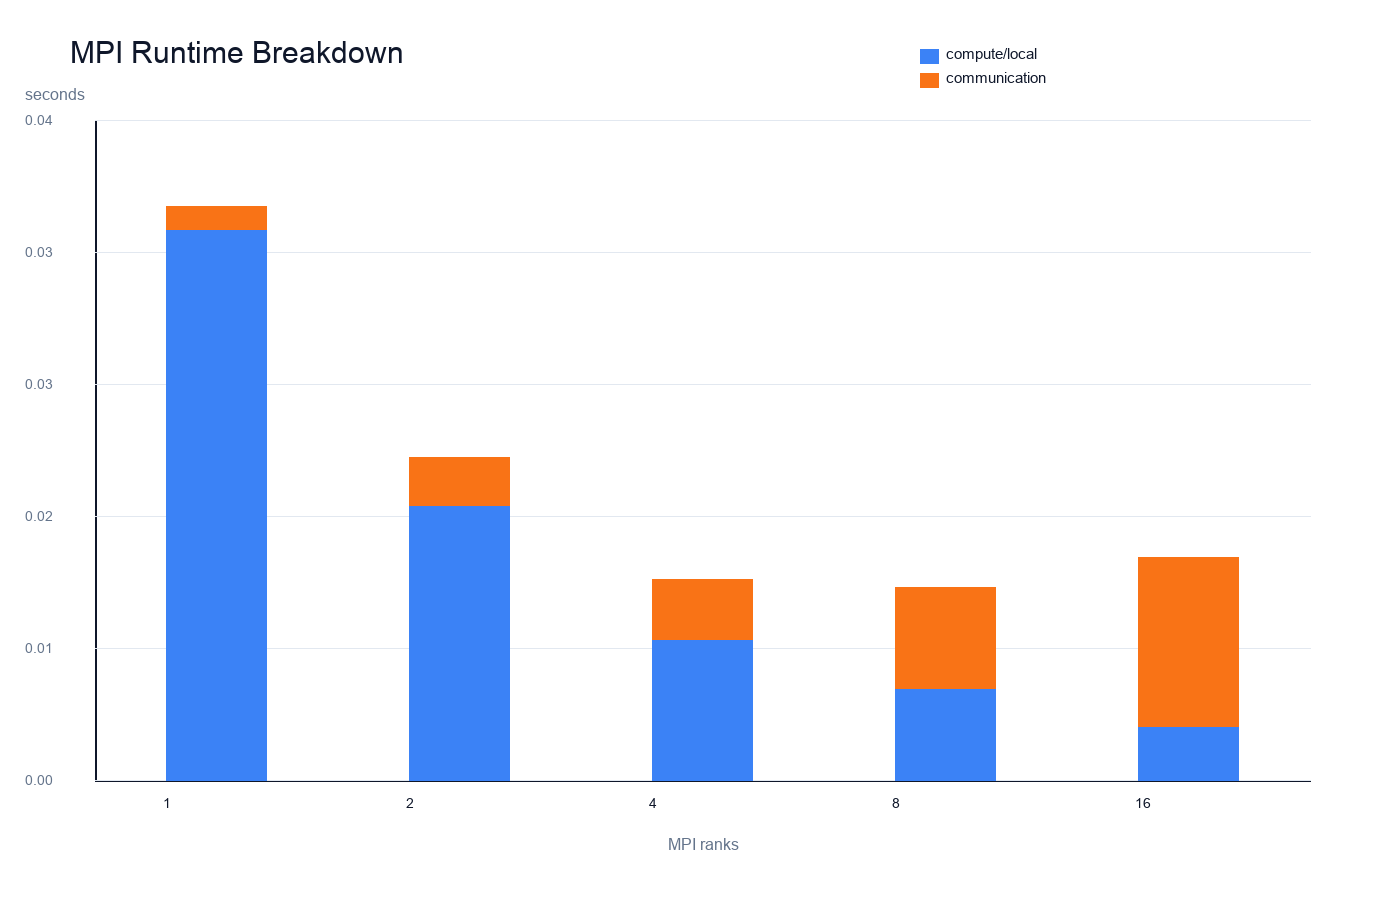
\includegraphics[width=0.48\textwidth]{results/figures/dardel_multinode_strong/mpi_runtime_breakdown.png}
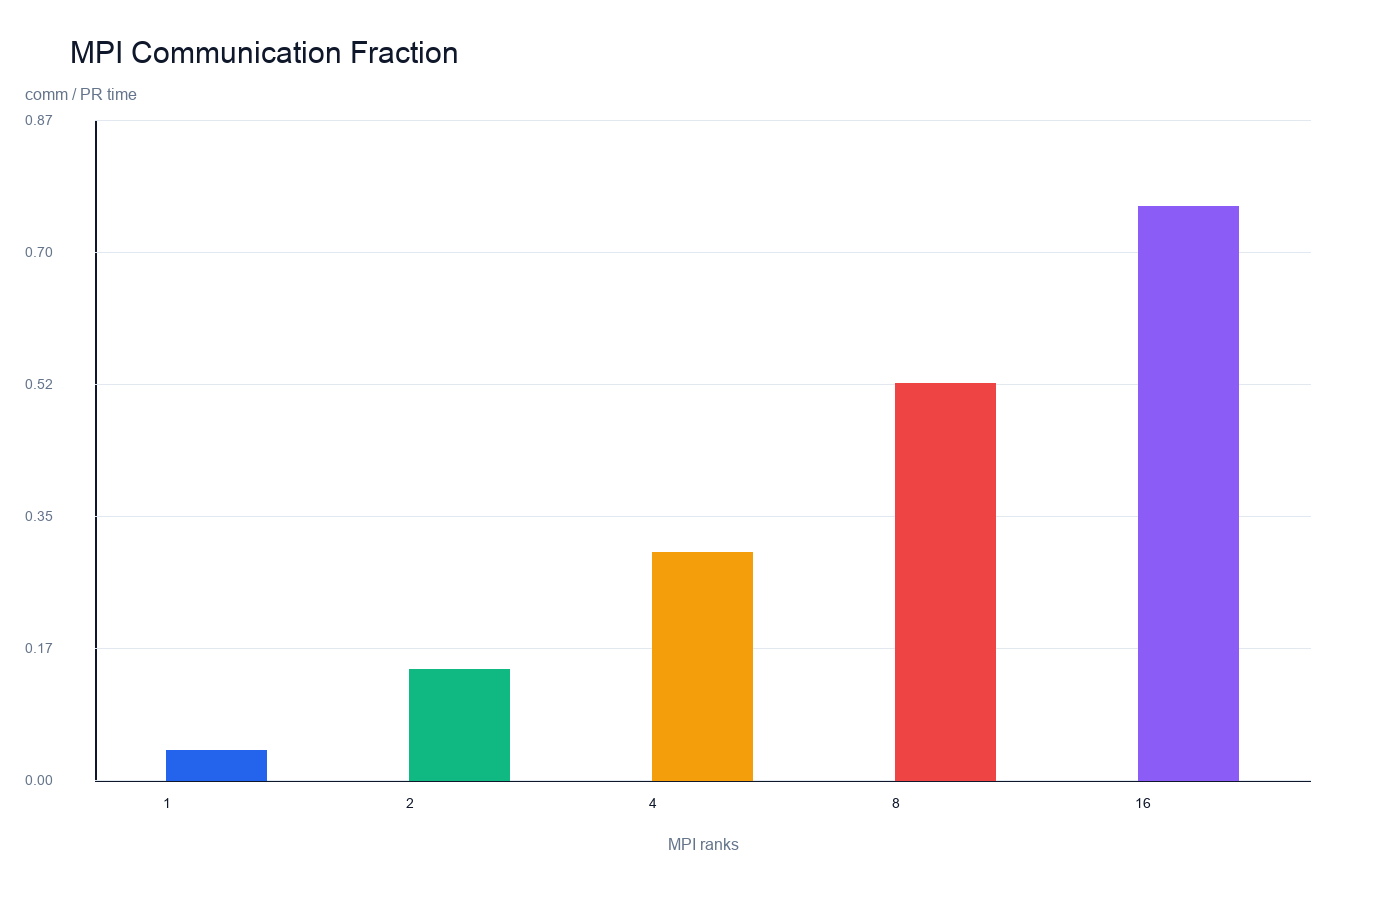
\includegraphics[width=0.48\textwidth]{results/figures/dardel_multinode_strong/mpi_comm_fraction.png}
\caption{Formal Dardel two-node runtime breakdown and communication
fraction on the synthetic graph.}
\label{fig:dardel-mpi-communication}
\end{figure}

\subsection{MPI Strong Scaling on the School Cluster}
\label{subsec:mpi-cluster-strong}

The school-cluster experiment exposes the same graph-size distinction.
The \texttt{polblogs.csv} graph is communication-bound, while the
larger synthetic graph scales to $P=4$ with $2.14\times$ speedup before
communication overtakes useful sparse work.

\begin{table}[H]
\centering
\caption{School-cluster MPI strong scaling on
\texttt{polblogs.csv} (directed), five repetitions per row.}
\label{tab:mpi-cluster-polblogs}
\small
\begin{tabular}{rrrrrr}
\toprule
Ranks & PR (s) & Comm frac. & Speedup & Efficiency & Imbalance \\
\midrule
1  & 0.001484 & 0.0142 & 1.000000 & 1.000000 & 1.000 \\
2  & 0.001889 & 0.8397 & 0.785472 & 0.392736 & 1.887 \\
4  & 0.002927 & 0.8878 & 0.506936 & 0.126734 & 3.129 \\
8  & 0.002461 & 0.9801 & 0.602844 & 0.075356 & 4.412 \\
16 & 0.002844 & 0.9898 & 0.521733 & 0.032608 & 4.536 \\
\bottomrule
\end{tabular}
\end{table}

\begin{table}[H]
\centering
\caption{School-cluster MPI strong scaling on
\texttt{synthetic\_100k\_1m.csv} (directed), five repetitions per row.}
\label{tab:mpi-cluster-synth}
\small
\begin{tabular}{rrrrrr}
\toprule
Ranks & PR (s) & Comm frac. & Speedup & Efficiency & Imbalance \\
\midrule
1  & 0.027228 & 0.0137 & 1.000000 & 1.000000 & 1.000 \\
2  & 0.017646 & 0.1766 & 1.543006 & 0.771503 & 1.035 \\
4  & 0.012738 & 0.4356 & 2.137590 & 0.534398 & 1.044 \\
8  & 0.015967 & 0.7505 & 1.705301 & 0.213163 & 1.047 \\
16 & 0.023347 & 0.8478 & 1.166240 & 0.072890 & 1.051 \\
\bottomrule
\end{tabular}
\end{table}

\begin{figure}[H]
\centering
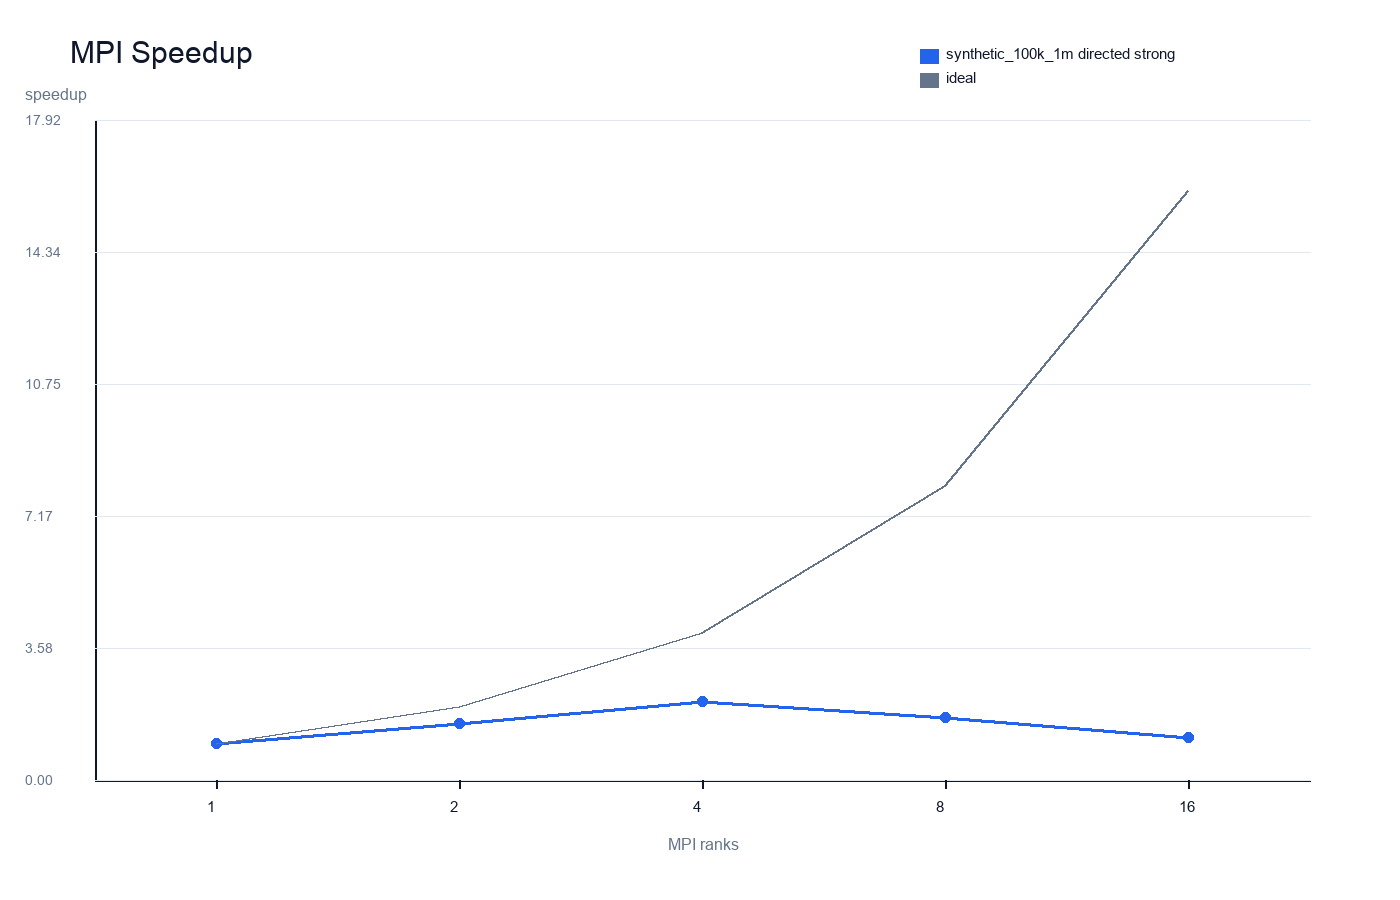
\includegraphics[width=0.48\textwidth]{results/figures/mpi_speedup_cluster.png}
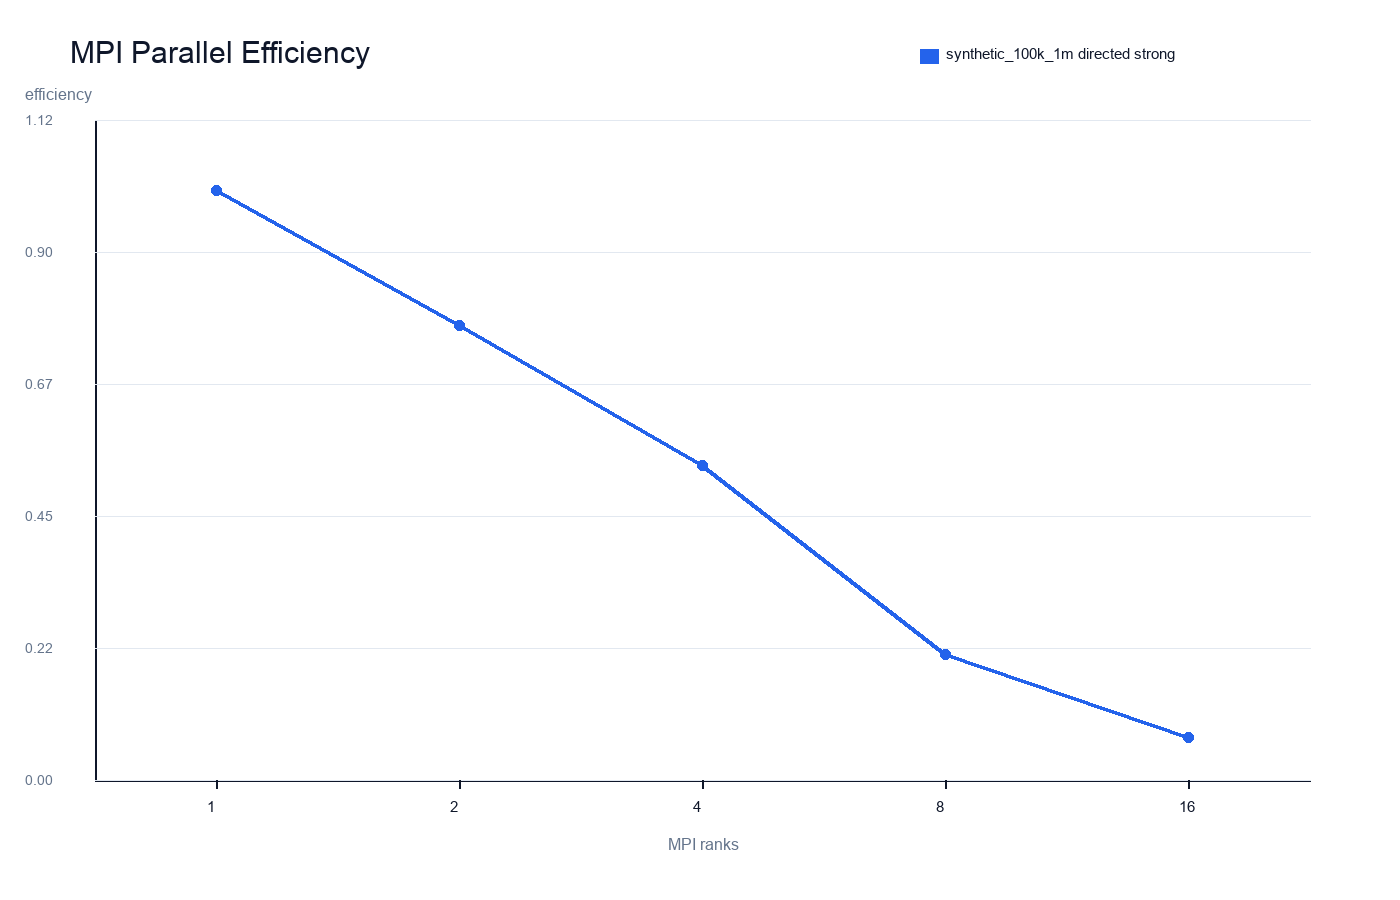
\includegraphics[width=0.48\textwidth]{results/figures/mpi_efficiency_cluster.png}
\caption{School-cluster MPI speedup and parallel efficiency on
\texttt{synthetic\_100k\_1m.csv}.}
\label{fig:cluster-mpi-speedup}
\end{figure}

\begin{figure}[H]
\centering
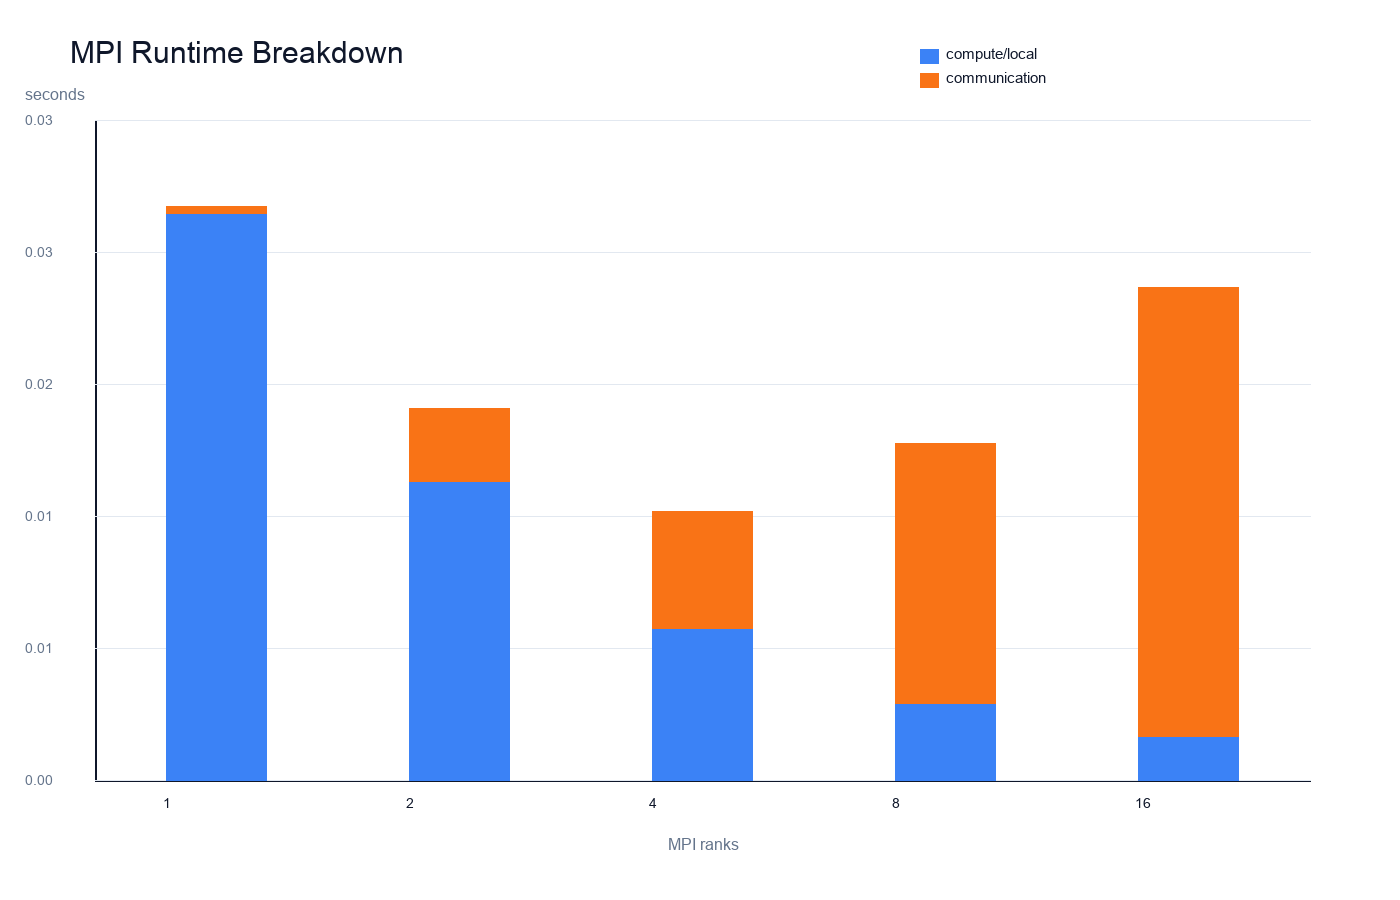
\includegraphics[width=0.48\textwidth]{results/figures/mpi_runtime_breakdown_cluster.png}
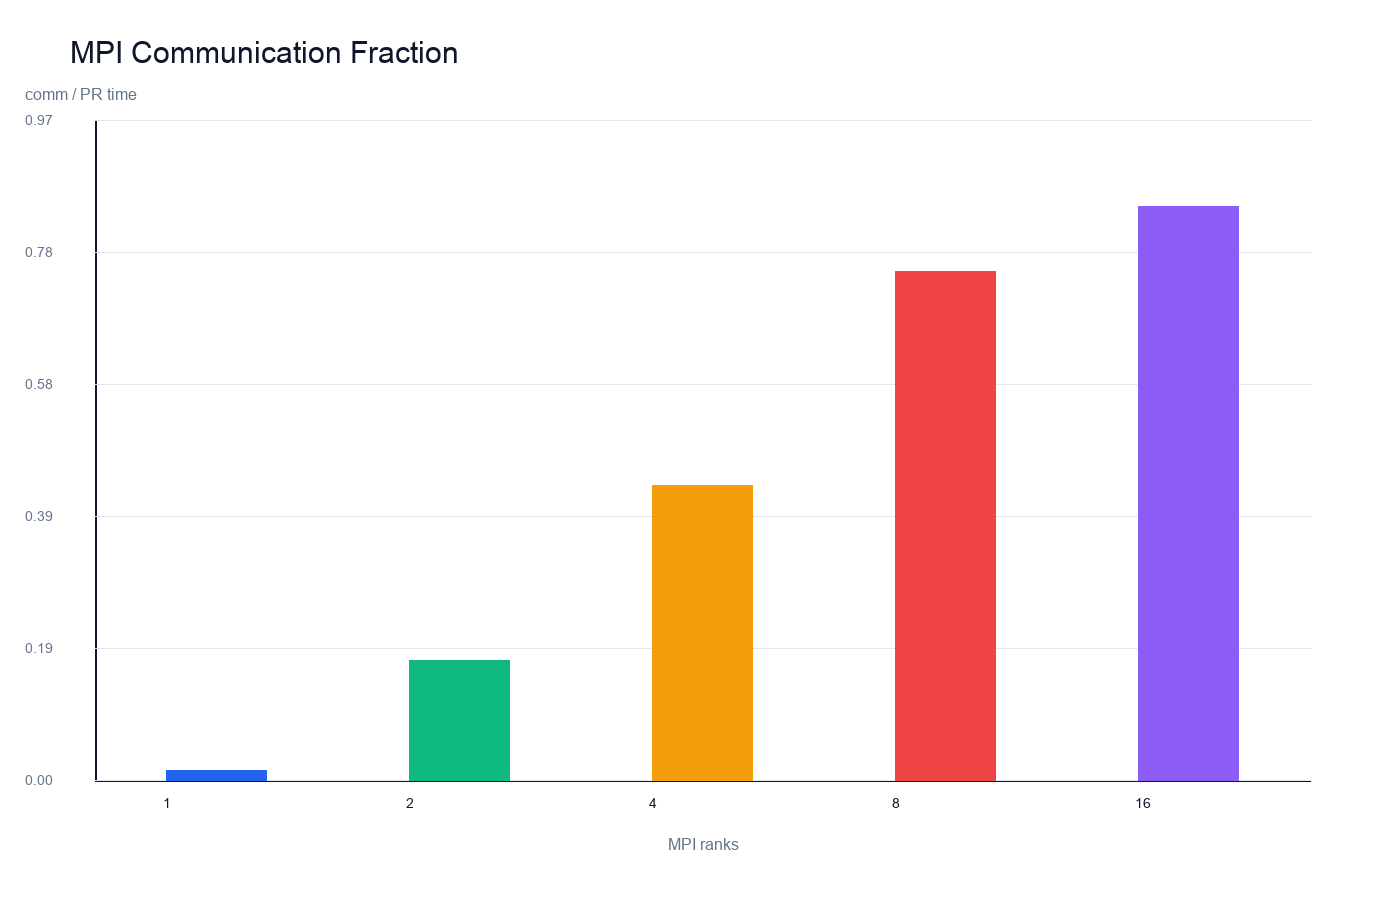
\includegraphics[width=0.48\textwidth]{results/figures/mpi_comm_fraction_cluster.png}
\caption{School-cluster MPI runtime breakdown and communication fraction
on the synthetic graph.}
\label{fig:cluster-mpi-communication}
\end{figure}

\subsection{MPI Weak Scaling on Dardel and the School Cluster}
\label{subsec:mpi-weak}

Weak scaling fixes per-rank work at $125\,000$ edges; the 16-rank
experiment consequently uses a $200\,000$-vertex,
$2\,000\,000$-edge synthetic graph. Both systems use the same
deterministically generated graph instances. Table~\ref{tab:mpi-weak}
shows that weak efficiency declines even while per-rank edge work is
fixed, because each iteration gathers a growing global PageRank vector.

\begin{table}[H]
\centering
\caption{MPI weak scaling with 125k edges per rank (five repetitions;
all rows pass verification).}
\label{tab:mpi-weak}
\small
\begin{tabular}{lrrrrr}
\toprule
Platform & Ranks & Nodes / Edges (k) & PR (s) & Comm frac. & Weak eff. \\
\midrule
Dardel (2 nodes) & 1  & 12.5 / 125  & 0.003778 & 0.0353 & 1.000000 \\
Dardel (2 nodes) & 2  & 25 / 250    & 0.005837 & 0.3138 & 0.647216 \\
Dardel (2 nodes) & 4  & 50 / 500    & 0.006134 & 0.3398 & 0.615899 \\
Dardel (2 nodes) & 8  & 100 / 1000  & 0.011932 & 0.5365 & 0.316600 \\
Dardel (2 nodes) & 16 & 200 / 2000  & 0.044137 & 0.5960 & 0.085593 \\
\midrule
Cluster & 1  & 12.5 / 125  & 0.003310 & 0.0123 & 1.000000 \\
Cluster & 2  & 25 / 250    & 0.005345 & 0.2442 & 0.619299 \\
Cluster & 4  & 50 / 500    & 0.007542 & 0.4821 & 0.438952 \\
Cluster & 8  & 100 / 1000  & 0.011587 & 0.5887 & 0.285695 \\
Cluster & 16 & 200 / 2000  & 0.024371 & 0.6814 & 0.135834 \\
\bottomrule
\end{tabular}
\end{table}

At 16 Dardel ranks, \texttt{MPI\_Allgatherv} alone averages
$0.020449$\,s of the $0.044137$\,s PageRank time; communication is
$59.60\%$ while imbalance remains only $1.051$. The school cluster is
faster in absolute time at 16 ranks but similarly loses weak efficiency,
with communication reaching $68.14\%$.

\begin{figure}[H]
\centering
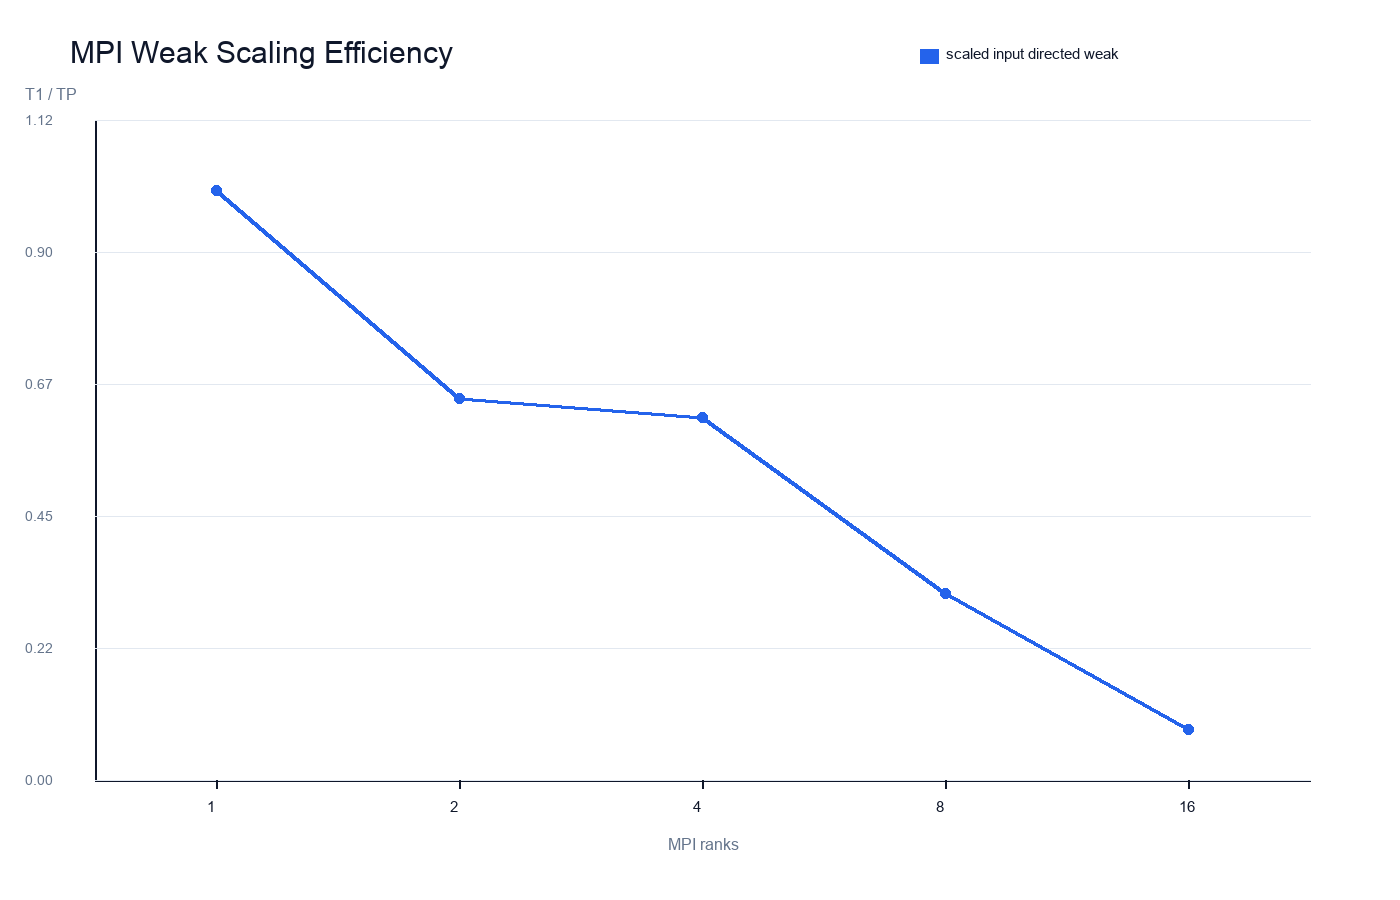
\includegraphics[width=0.48\textwidth]{results/figures/dardel_multinode_weak/mpi_weak_efficiency.png}
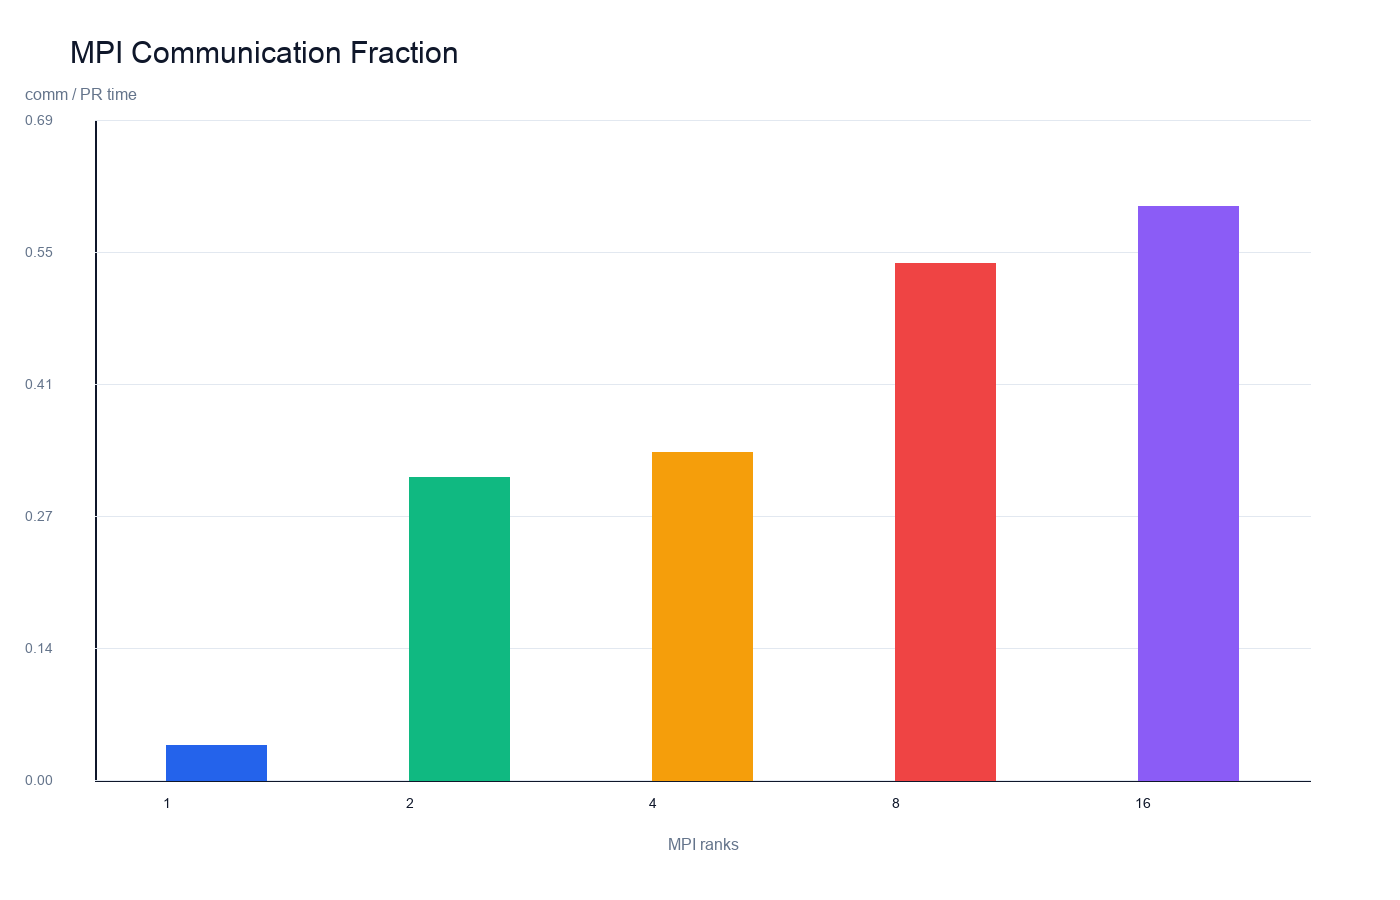
\includegraphics[width=0.48\textwidth]{results/figures/dardel_multinode_weak/mpi_comm_fraction.png}\\
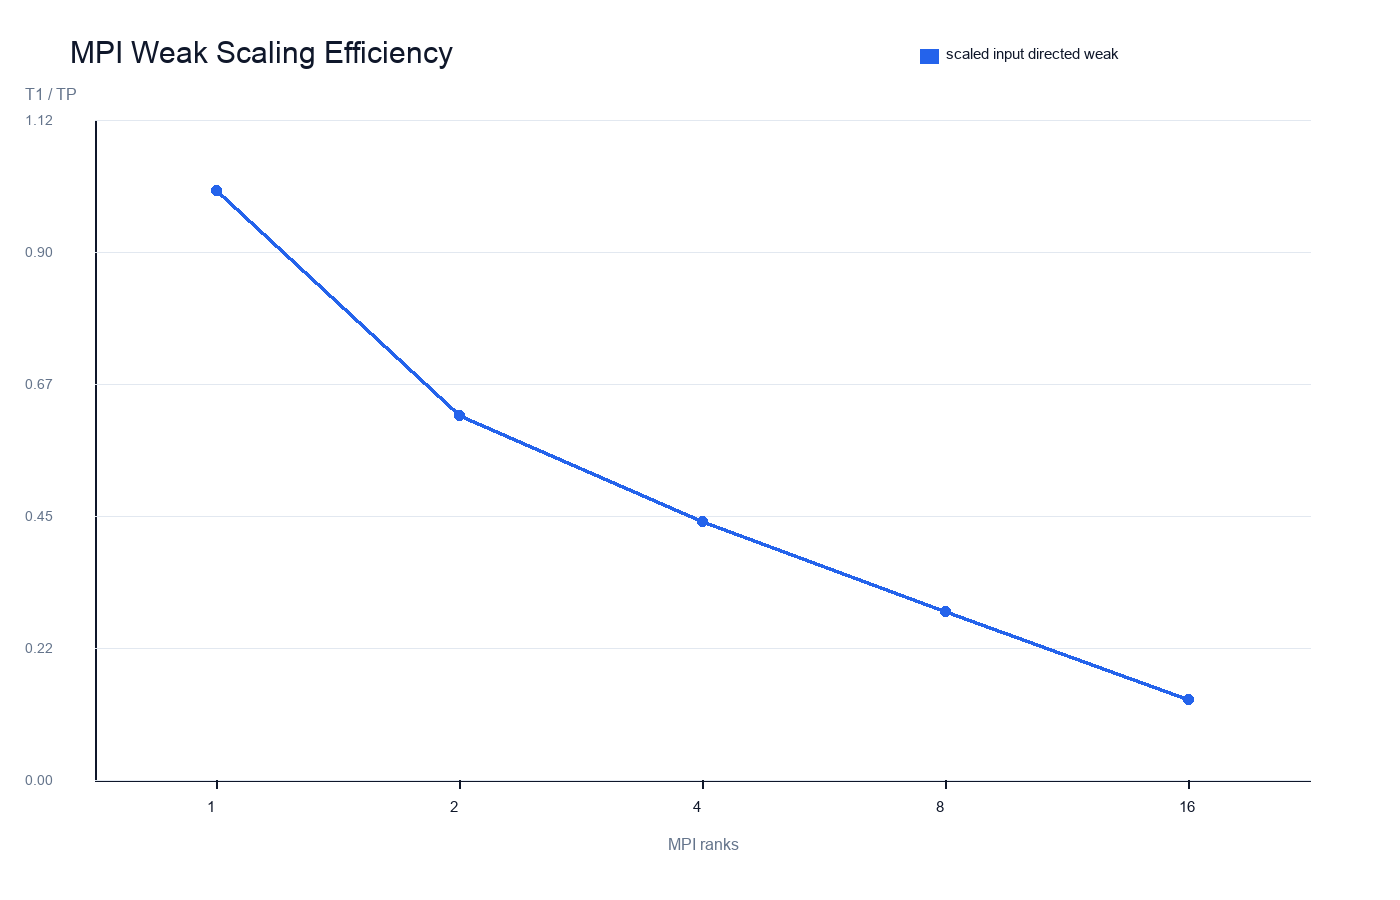
\includegraphics[width=0.48\textwidth]{results/figures/cluster_weak/mpi_weak_efficiency.png}
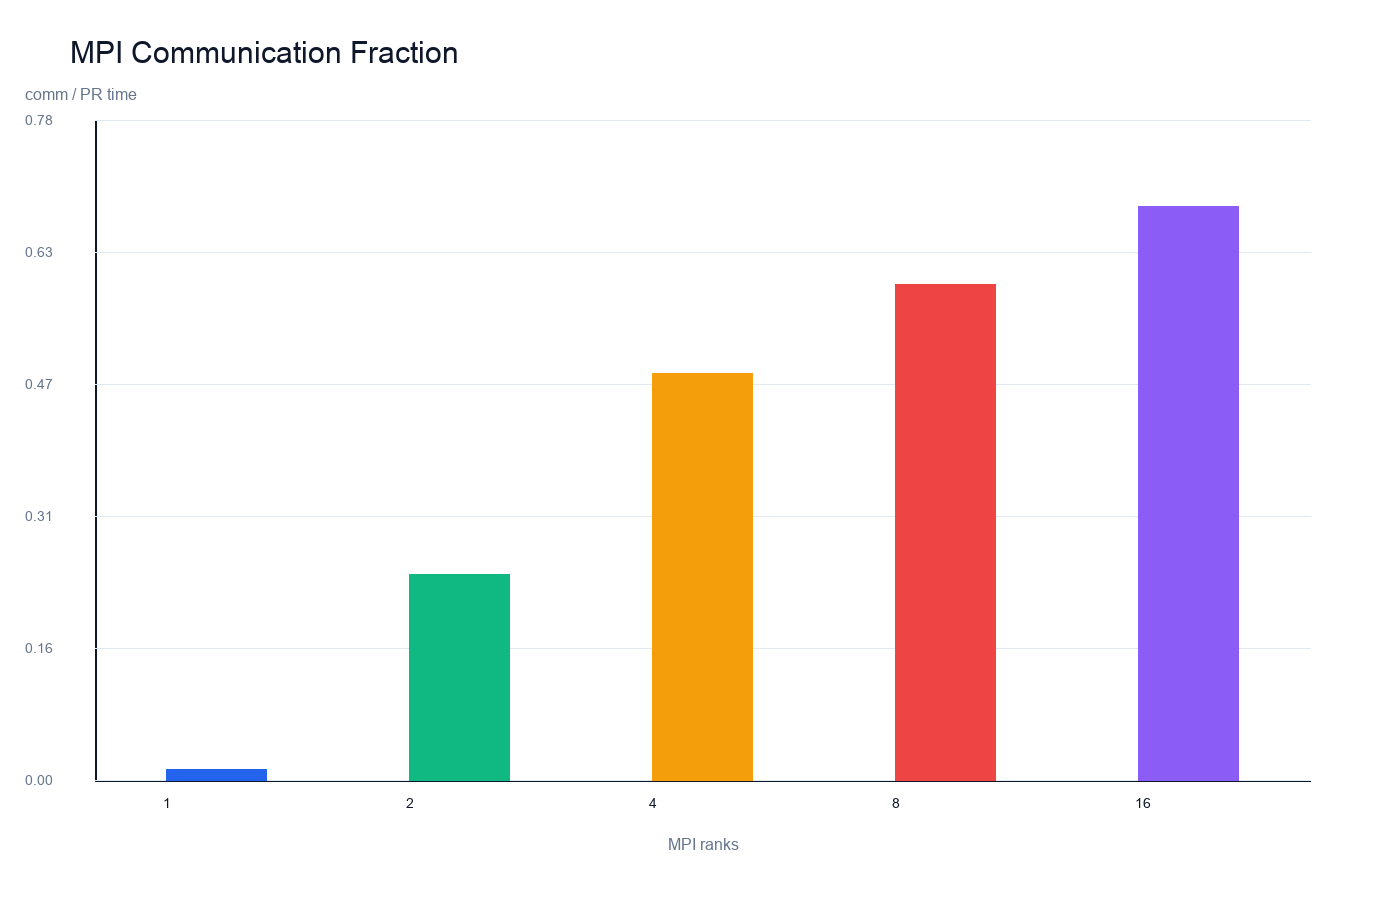
\includegraphics[width=0.48\textwidth]{results/figures/cluster_weak/mpi_comm_fraction.png}
\caption{Weak-scaling efficiency and communication fraction on formal
Dardel two-node runs (top) and the school cluster (bottom).}
\label{fig:weak-scaling}
\end{figure}

\subsection{OpenMP Strong Scaling on Three Systems}
\label{subsec:openmp-three}

The OpenMP binary was run on all three CPU platforms at thread counts
$T{=}1,\dots,64$ with five back-to-back repetitions per cell.
Table~\ref{tab:openmp-three-systems} reports the average PR-kernel time
on the \path{synthetic_100k_1m.csv} graph; millisecond-scale
\texttt{polblogs} results fall inside the per-platform noise floor.

\begin{table}[H]
\centering
\caption{OpenMP strong scaling on \texttt{synthetic\_100k\_1m.csv}
(directed). PR time in ms, speedup vs.\ $T{=}1$; per-platform best in bold.}
\label{tab:openmp-three-systems}
\small
\begin{tabular}{r rr rr rr}
\toprule
 & \multicolumn{2}{c}{Colab (2 vCPU)} & \multicolumn{2}{c}{KTH (112 cores)} & \multicolumn{2}{c}{Dardel (128 cores)} \\
\cmidrule(lr){2-3}\cmidrule(lr){4-5}\cmidrule(lr){6-7}
T & PR (ms) & Speedup & PR (ms) & Speedup & PR (ms) & Speedup \\
\midrule
1  & 107.97 & 1.00          & 34.67  & 1.00          & 33.88 & 1.00 \\
2  & 128.53 & 0.84          & 23.41  & 1.48          & 18.97 & 1.79 \\
4  & 84.79  & 1.27$^\ast$   & 14.08  & 2.46          & 11.70 & 2.90 \\
8  & ---    & ---           &  9.72  & 3.57          &  9.03 & 3.75 \\
16 & ---    & ---           & 12.41  & 2.79          & \textbf{7.85} & \textbf{4.32} \\
32 & ---    & ---           & \textbf{7.75} & \textbf{4.48} &  8.92 & 3.80 \\
64 & ---    & ---           & 18.96 & 1.83          & 13.10 & 2.59 \\
\bottomrule
\end{tabular}
\\[2pt]
\footnotesize $^\ast$Colab has 2 vCPU; $T{=}4$ is oversubscribed.
\end{table}

All three platforms saturate near $4$--$4.5\times$ peak speedup despite
up to $128$ physical cores being available, matching the bandwidth
ceiling predicted by the $0.10$ FLOP/Byte arithmetic intensity. KTH
recovers from a dip at $T{=}16$ at $T{=}32$, while Dardel scales to a
$T{=}16$ peak. Colab's two vCPUs contend for cache and bandwidth on
the random read pattern, so oversubscribed results are not useful
scaling evidence.

\section{Optimization Effectiveness}
\label{sec:wang-optimization}

The first profiling-guided optimization precomputes
\texttt{inv\_out\_degree[u]} during graph construction so that the
PageRank inner loop multiplies rather than performs a floating-point
division per incoming-edge contribution:
\[
s_v = \sum_{u\in In(v)} pr_u \cdot \texttt{inv\_out\_degree[u]}.
\]
The second optimization applies \texttt{schedule(dynamic, 256)} to the
hybrid sparse-update loop so destinations with unequal incoming-edge
counts can be redistributed between threads.

The formal ablation profiler constructs four hybrid variants:
\path{no_inv_static}, \path{inv_static}, \path{no_inv_dynamic}, and
\path{inv_dynamic}. It was run on the school-cluster CPU server with
OpenMPI core binding enabled; one warmup precedes ten
correctness-checked repetitions per layout. It records both PageRank
time and sparse-update-kernel time, as well as thread-level processed
edge counts with imbalance metric $\max_t M_t/\overline{M_t}$.
Efficiency is computed per variant from that variant's \texttt{1x1}
baseline.

\begin{table}[H]
\centering
\caption{Formal optimization evidence on the regular synthetic graph.
PR and update times are seconds; efficiency uses each variant's own
\texttt{1x1} baseline.}
\label{tab:wang-optimization-ablation}
\scriptsize
\begin{tabular}{lrrrrrrr}
\toprule
Config & PR before & PR full opt. & Speedup & Update before & Update full opt. & $E$ before & $E$ full opt. \\
\midrule
\texttt{1x1}  & 0.035842 & 0.032455 & 1.1043 & 0.033078 & 0.029548 & 1.0000 & 1.0000 \\
\texttt{1x4}  & 0.012826 & 0.010960 & 1.1702 & 0.010691 & 0.008779 & 0.6986 & \textbf{0.7403} \\
\texttt{1x8}  & 0.006531 & 0.006945 & 0.9403 & 0.004768 & 0.004852 & \textbf{0.6860} & 0.5841 \\
\texttt{1x16} & 0.005576 & 0.005765 & 0.9672 & 0.003683 & 0.002765 & \textbf{0.4017} & 0.3518 \\
\texttt{2x8}  & 0.006187 & 0.005274 & 1.1732 & 0.003532 & 0.002912 & 0.3621 & \textbf{0.3846} \\
\texttt{4x4}  & 0.007609 & 0.007524 & 1.0113 & 0.003938 & 0.003026 & \textbf{0.2944} & 0.2696 \\
\bottomrule
\end{tabular}
\end{table}

\begin{table}[H]
\centering
\caption{Dynamic-scheduling evidence on the controlled skewed graph:
\texttt{inv\_static} versus \texttt{inv\_dynamic}.}
\label{tab:wang-optimization-skewed}
\small
\begin{tabular}{lrrrrr}
\toprule
Config & Static imbalance & Dynamic imbalance & Reduction & Static update (s) & Dynamic update (s) \\
\midrule
\texttt{1x4}  & 3.1591  & 1.1489 & 2.750$\times$ & 0.028158 & 0.010108 \\
\texttt{1x8}  & 6.0388  & 1.2420 & 4.862$\times$ & 0.020228 & 0.005293 \\
\texttt{1x16} & 11.7988 & 1.2415 & 9.504$\times$ & 0.017573 & 0.003117 \\
\bottomrule
\end{tabular}
\end{table}

On the regular graph, the full optimization improves PR time at
\texttt{1x1}, \texttt{1x4}, and \texttt{2x8}, but does not universally
improve highly threaded end-to-end time because synchronization and
scheduling overhead can offset reduced update-kernel time. The skewed
stress input isolates the schedule benefit: at \texttt{1x16}, dynamic
scheduling reduces measured thread imbalance from $11.7988$ to $1.2415$
and update time from $0.017573$\,s to $0.003117$\,s.

\begin{figure}[H]
\centering
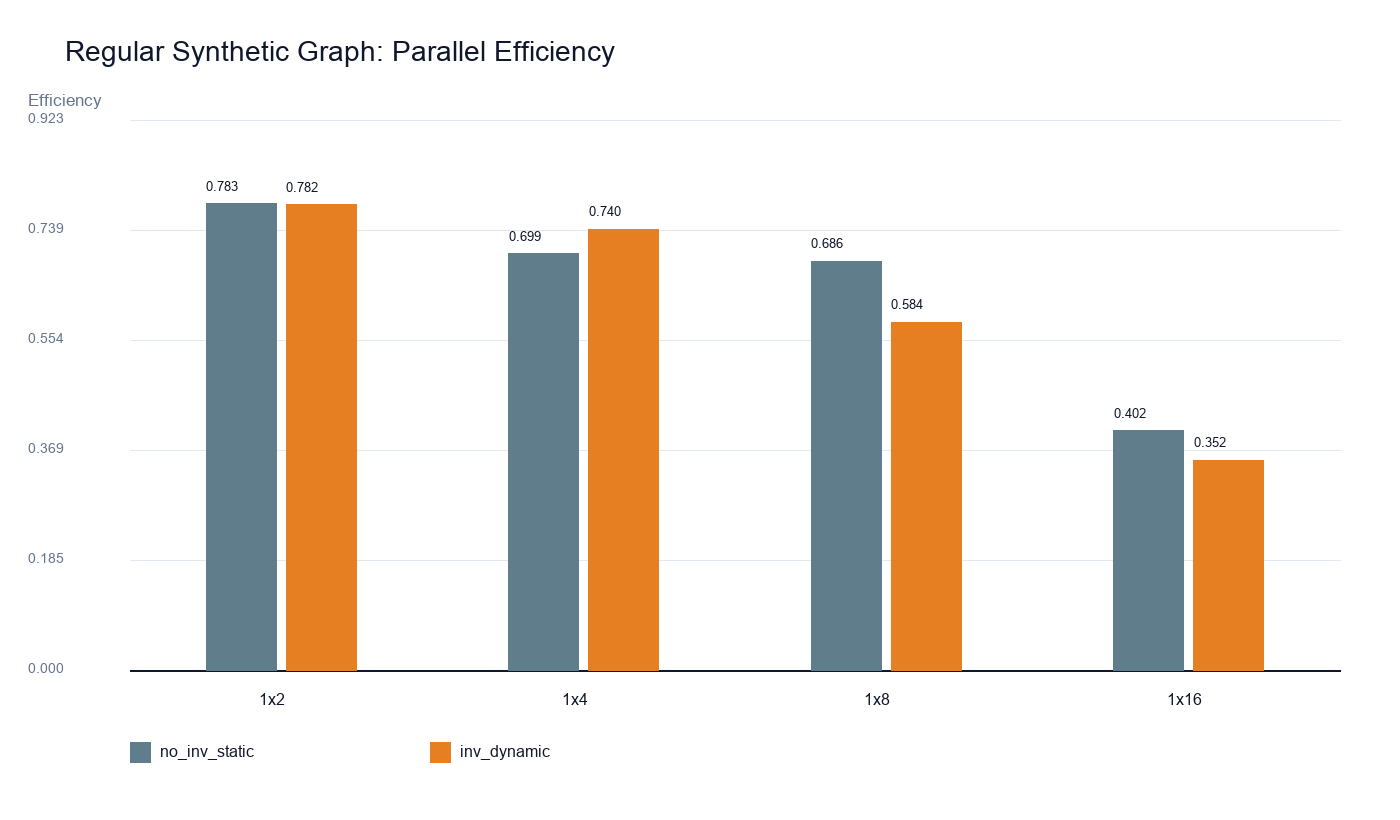
\includegraphics[width=0.48\textwidth]{results/figures/cluster_optimization/optimization_efficiency.png}
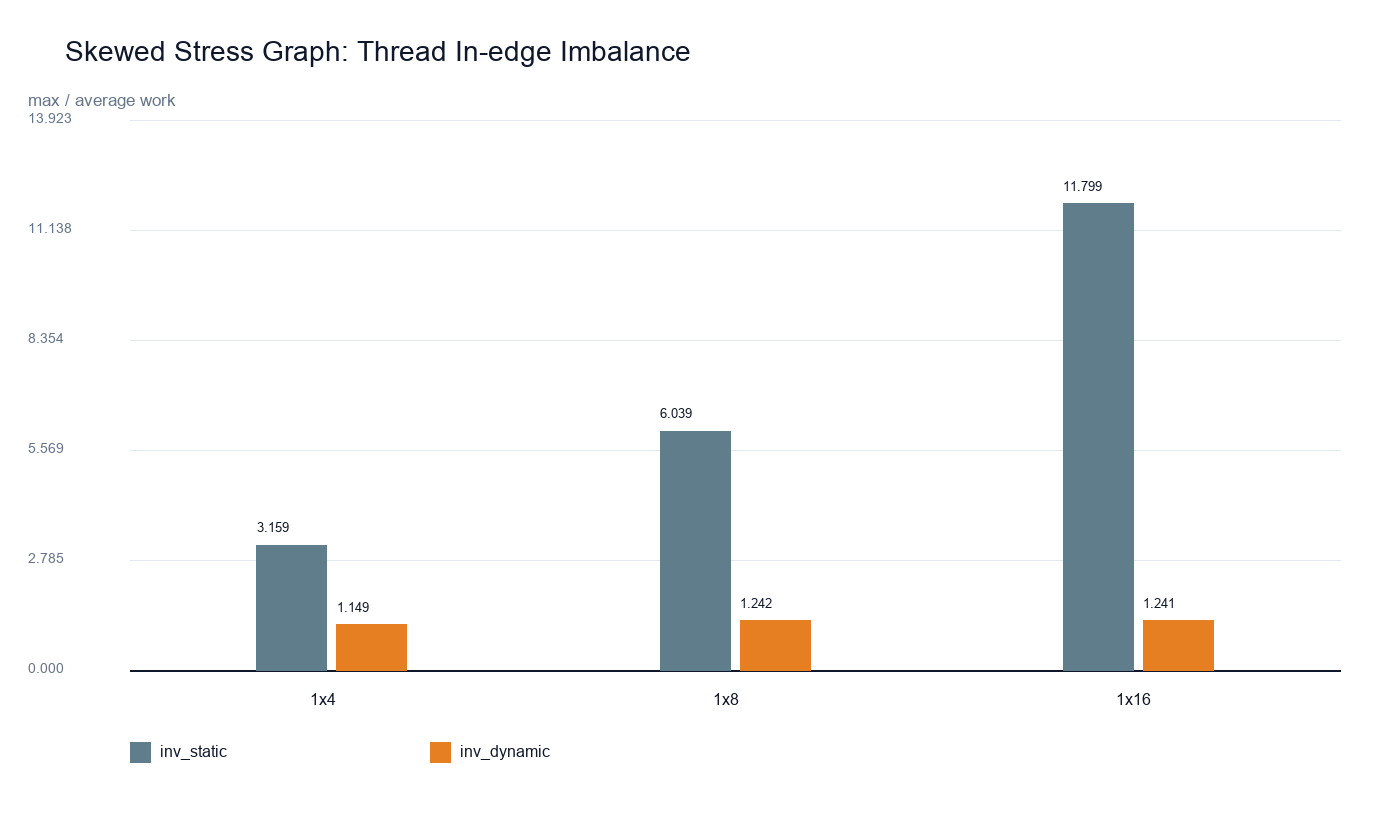
\includegraphics[width=0.48\textwidth]{results/figures/cluster_optimization/optimization_thread_imbalance.png}
\caption{Formal CPU optimization evidence: before/after parallel
efficiency on the regular graph (left) and static versus dynamic thread
imbalance on the skewed graph (right).}
\label{fig:wang-optimization-evidence}
\end{figure}

\subsection{Confirmed-Device GPU Offloading Comparison}
\label{subsec:gpu-results}

OpenMP target execution was confirmed on the DD2356 Small GPU server,
which exposed one NVIDIA H100 \texttt{MIG 1g.10gb} target device. On
\texttt{synthetic\_100k\_1m.csv}, retaining arrays across PageRank
iterations reduces average PR time from $0.059829$\,s for naive mapping
to $0.033684$\,s for persistent mapping, a $1.7762\times$ improvement.
Persistent offload is slightly faster than the single-CPU serial
reference for the kernel metric, but a Hybrid \texttt{4x2} control on
the same server completes in $0.010364$\,s and is $3.2500\times$ faster
than persistent offload at this graph size.

\begin{table}[H]
\centering
\caption{Confirmed-device GPU comparison on the DD2356 Small GPU server
for \texttt{synthetic\_100k\_1m.csv} (directed), five-run averages.}
\label{tab:wang-gpu-comparison}
\small
\begin{tabular}{lllr}
\toprule
Variant & Configuration & PR time (s) & Correctness \\
\midrule
Serial & 1 CPU thread & 0.036452 & reference \\
OpenMP target GPU & naive mapping & 0.059829 & PASS, device verified \\
OpenMP target GPU & persistent mapping & \textbf{0.033684} & PASS, device verified \\
Hybrid MPI+OpenMP & \texttt{4x2}, 8 CPU workers & \textbf{0.010364} & PASS \\
\bottomrule
\end{tabular}
\end{table}

\begin{figure}[H]
\centering
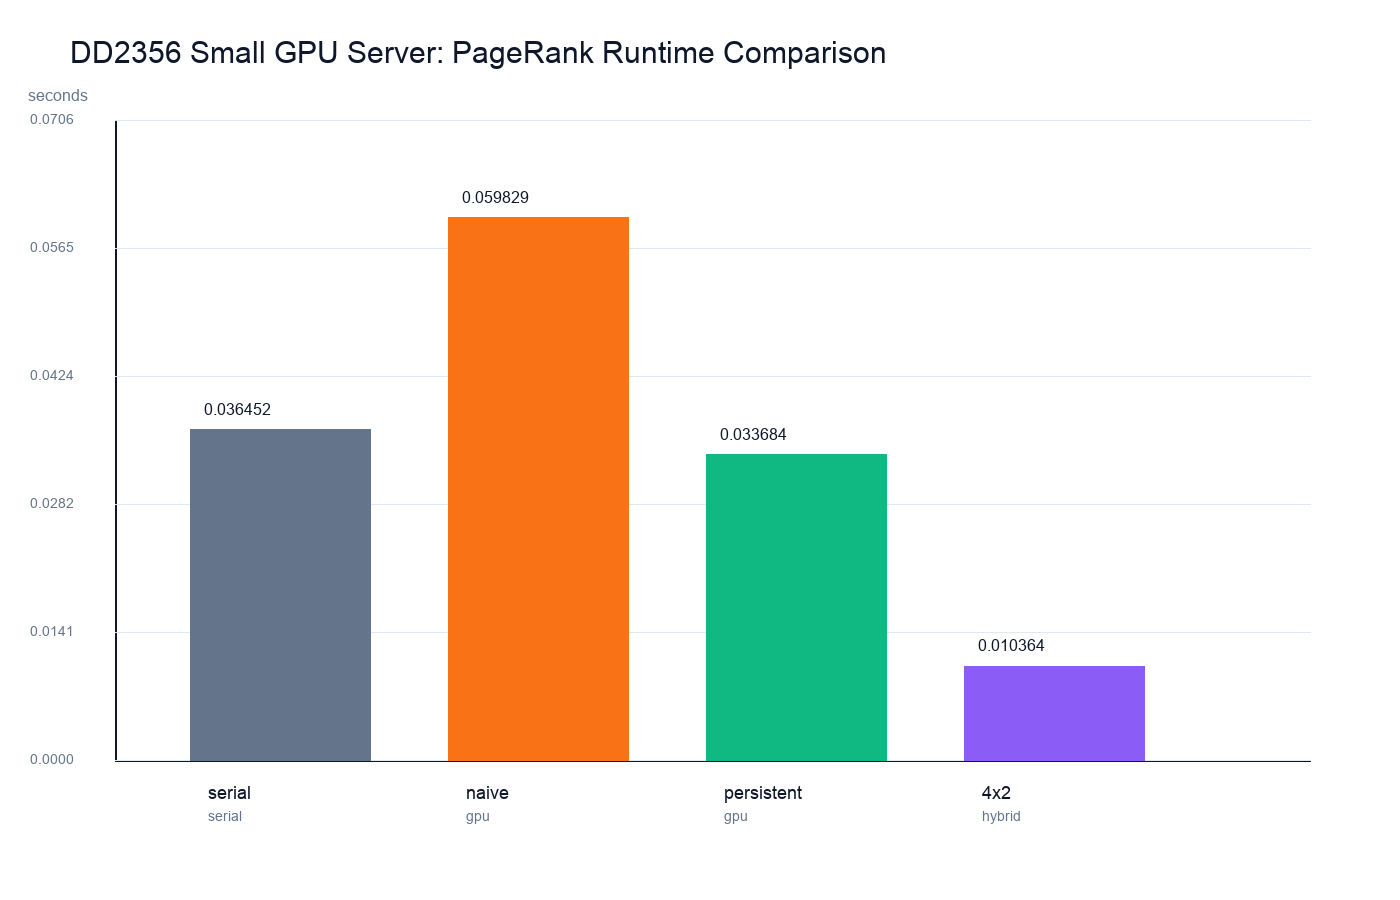
\includegraphics[width=0.48\textwidth]{results/figures/cluster_gpu/gpu_pr_time_comparison.png}
\hfill
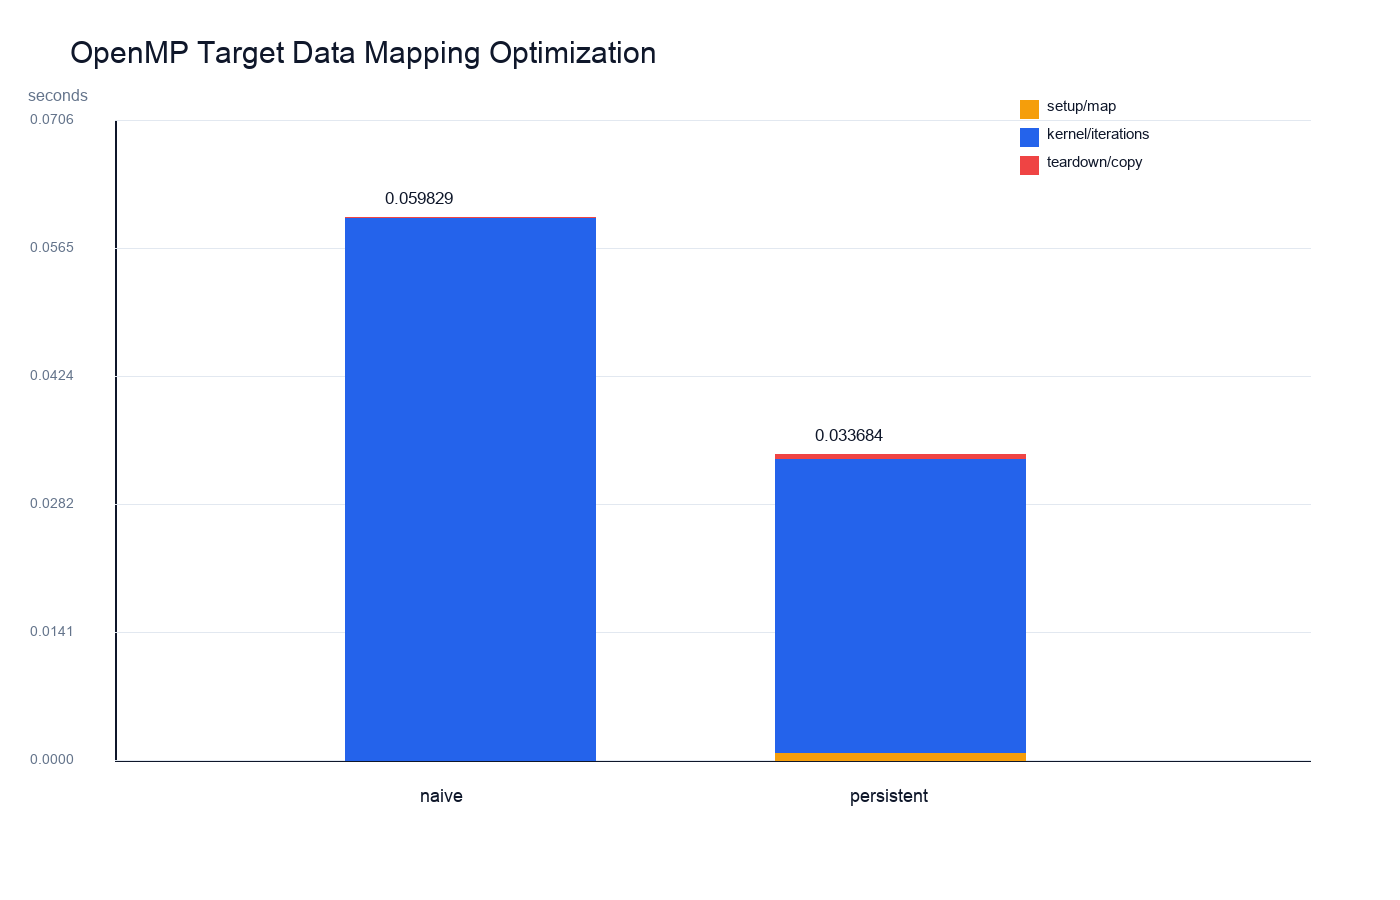
\includegraphics[width=0.48\textwidth]{results/figures/cluster_gpu/gpu_mapping_breakdown.png}
\caption{Same-server GPU and Hybrid timing comparison (left) and OpenMP
target mapping optimization breakdown (right).}
\label{fig:wang-gpu-comparison}
\end{figure}

\subsection{School-Cluster Fixed-Worker Hybrid Sweep}
\label{subsec:hybrid-fixed}

The formal fixed-worker hybrid runs keep $P\!\times\!N=16$ CPU workers
on the school cluster while varying MPI ranks and threads per rank. For
\texttt{polblogs.csv}, the tiny per-rank workload favours
\texttt{16x1}; for the larger synthetic graph the best average result is
\texttt{4x4}, which exposes MPI parallelism without yet maximising
collective cost.

\begin{table}[H]
\centering
\caption{Hybrid fixed-16-worker sweep on the school cluster for
\texttt{polblogs.csv} (directed).}
\label{tab:wang-hybrid-polblogs}
\small
\begin{tabular}{rrrrrr}
\toprule
Ranks & Threads/rank & PR (s) & Comm frac. & Speedup vs.\ \texttt{1x16} & Status \\
\midrule
1  & 16 & 0.024310 & 0.0018 & 1.0000 & PASS \\
2  & 8  & 0.010850 & 0.1643 & 2.2406 & PASS \\
4  & 4  & 0.005325 & 0.7428 & 4.5652 & PASS \\
8  & 2  & 0.004281 & 0.8655 & 5.6783 & PASS \\
16 & 1  & \textbf{0.002907} & 0.9533 & \textbf{8.3631} & PASS \\
\bottomrule
\end{tabular}
\end{table}

\begin{table}[H]
\centering
\caption{Hybrid fixed-16-worker sweep on the school cluster for
\texttt{synthetic\_100k\_1m.csv} (directed).}
\label{tab:wang-hybrid-synth}
\small
\begin{tabular}{rrrrrr}
\toprule
Ranks & Threads/rank & PR (s) & Comm frac. & Speedup vs.\ \texttt{1x16} & Status \\
\midrule
1  & 16 & 0.036692 & 0.0137 & 1.0000 & PASS \\
2  & 8  & 0.018884 & 0.1758 & 1.9431 & PASS \\
4  & 4  & \textbf{0.011843} & 0.6741 & \textbf{3.0981} & PASS \\
8  & 2  & 0.019373 & 0.7682 & 1.8940 & PASS \\
16 & 1  & 0.012234 & 0.8220 & 2.9992 & PASS \\
\bottomrule
\end{tabular}
\end{table}

\subsection{Additional Multi-Budget Hybrid Measurements}
\label{subsec:hybrid-multi}

The group also collected multi-budget hybrid measurements on
\texttt{synthetic\_100k\_1m.csv}. The KTH rows below complement the
formal fixed-16-worker evidence by sampling $W=4$ and $W=8$. The
Dardel entries were re-measured with clean CPU placement on a dedicated
allocation. Their passing $W=4,8,16$ rows therefore provide formal
hybrid comparison evidence; for $W=32$, the pure-MPI \texttt{(32,1)}
row failed verification and is excluded from all slowdown claims.

\begin{table}[H]
\centering
\caption{Best $(P,N)$ splits by CPU-worker budget $W$ on the school
cluster and in clean Dardel hybrid re-measurements. A failed validation
row is excluded from comparison.}
\label{tab:hybrid-multi-budget}
\small
\begin{tabular}{lr lrr rr}
\toprule
Platform & $W$ & Best & PR (ms) & comm \% & Pure-MPI $(P,1)$ PR (ms) & Slowdown \\
\midrule
KTH    & 4  & $(2,2)$  & 16.79 & 15.7 &     34.33 &     $2.0\times$ \\
KTH    & 8  & $(2,4)$  & 16.31 & 16.0 &  3\,689.26 &   $226\times$ \\
Dardel & 4  & $(1,4)$  & 16.97 &  7.6 & 12\,385.23 &   $730\times$ \\
Dardel & 8  & $(1,8)$  & 10.28 &  8.2 & 11\,675.67 & $1\,136\times$ \\
Dardel & 16 & $(1,16)$ & 10.19 & 27.5 & 17\,886.36 & $1\,756\times$ \\
Dardel & 32 & $(1,32)$ & 10.18 & 28.0 & \multicolumn{2}{c}{\texttt{(32,1)} excluded (FAIL)} \\
\bottomrule
\end{tabular}
\end{table}

The KTH multi-budget samples support using a small MPI-rank count within
a shared-memory node. The clean Dardel measurements instead select
single-rank OpenMP layouts at every tested worker budget, consistent
with the high collective cost observed in the formally placed Dardel
two-node MPI measurements. The failing \texttt{(32,1)} sample is
reported for auditability only and contributes no performance claim.

\section{Discussion}
\label{sec:discussion}

The measurements identify two related but distinct limits. Within a
shared-memory CPU node, the $0.10$ FLOP/Byte kernel reaches a bandwidth
ceiling: OpenMP peaks near $4$--$4.5\times$ despite far more physical
cores. Across MPI ranks, full-vector \texttt{MPI\_Allgatherv} becomes
the binding cost. In the formal Dardel two-node experiment this does
not prevent useful scaling on the balanced one-million-edge graph:
speedup reaches $2.98\times$ at eight ranks. It does, however, suppress
efficiency by 16 ranks and eliminates benefit immediately for
millisecond-scale \texttt{polblogs}. Weak scaling exhibits the same
growing-vector cost even though the local edge budget is fixed.

The optimization and accelerator experiments refine that conclusion.
Reciprocal out-degree caching and dynamic scheduling reduce local work
cost when there is enough computation or controlled in-degree skew; on
the skewed graph dynamic scheduling reduces measured thread imbalance
by $9.504\times$ at \texttt{1x16}. Persistent GPU mapping similarly
eliminates repeated mapping overhead and improves naive offloading by
$1.7762\times$, confirming that data movement was an avoidable GPU
cost. At the measured one-million-edge scale, however, a same-server
hybrid CPU configuration still outperforms the GPU path. The next
algorithmic step is therefore communication reduction, such as a graph
partition that exchanges required boundary contributions rather than a
full PageRank vector each iteration.

\section{Conclusion}
\label{sec:conclusion}

We implemented and evaluated serial, OpenMP, MPI, hybrid MPI+OpenMP,
and confirmed-device OpenMP GPU PageRank variants. Serial profiling
places the kernel at $0.10$ FLOP/Byte, predicting the memory-bound
behaviour observed in OpenMP scaling, where Dardel reaches a
$4.32\times$ peak at $T=16$. Formal two-node Dardel MPI measurements
show useful strong scaling for a balanced synthetic graph up to
$2.98\times$ at $P=8$, followed by declining efficiency as
\texttt{MPI\_Allgatherv} grows; small graphs and weak-scaling runs make
the same communication limitation more visible. Formal optimization
evidence demonstrates substantial thread-balance gains on a skewed
input, and confirmed H100 MIG execution shows persistent target data
mapping is $1.7762\times$ faster than naive offloading, although the
same-server Hybrid \texttt{4x2} control remains $3.2500\times$ faster
at the tested graph size. All formal-result variants verify within
$10^{-6}$ of the serial reference. Replacing replicated-vector exchange
with communication-reduced graph partitioning is the clearest route to
further scalable performance.

\section*{Contributions}
\label{sec:contrib}

\noindent\textbf{Pengyu Wang.}
Pengyu Wang implemented the MPI decomposition and communication timing,
ran and analysed the formal Dardel multi-node and school-cluster MPI
strong/weak-scaling experiments, added the 16-rank weak-scaling workflow
with dynamically sized graph readers, and integrated the MPI result
pipeline. He implemented and measured OpenMP GPU offloading, including
the persistent-device-data optimization and confirmed H100 MIG
execution, and completed the formal CPU ablation for reciprocal
out-degree caching and dynamic scheduling with thread-imbalance and
parallel-efficiency measurements.

% TODO before final submission: Jiachen Shi and Minyi Zhu must add their
% confirmed contribution paragraphs here; do not infer individual claims
% solely from result tables.

\begin{thebibliography}{9}
    \bibitem{pagerank} L. Page, S. Brin, R. Motwani, and T. Winograd,
    ``The PageRank Citation Ranking: Bringing Order to the Web,''
    Stanford InfoLab Technical Report, 1999.

    \bibitem{openmp} OpenMP Architecture Review Board, ``OpenMP
    Application Programming Interface, Version 5.2,'' Nov.\ 2021.

    \bibitem{mpi} Message Passing Interface Forum, ``MPI: A
    Message-Passing Interface Standard, Version 4.0,'' Jun.\ 2021.

    \bibitem{snap} J. Leskovec and A. Krevl, ``SNAP Datasets: Stanford
    Large Network Dataset Collection,'' \url{http://snap.stanford.edu/data},
    2014.

    \bibitem{dardel} PDC Center for High Performance Computing,
    ``Dardel system documentation,''
    \url{https://www.pdc.kth.se/hpc-services/computing-systems/dardel-1.1043529},
    accessed May 2026.

    \bibitem{gprof} S. L. Graham, P. B. Kessler, and M. K. McKusick,
    ``gprof: A Call Graph Execution Profiler,'' \emph{Proc. SIGPLAN
    Symp. on Compiler Construction}, 1982, pp.\ 120--126.

    \bibitem{perf} A. C. de Melo, ``The New Linux `perf' Tools,''
    \emph{Linux Kongress}, 2010.
\end{thebibliography}

\end{document}
